\section{Experiments}
%\section{Experiments}
%\label{sec:experiments}
%
%\subsection{Simulated Imagery}
%\label{ssec:simulated}
%
%\subsection{Real Imagery}
%\label{ssec:real}
%
%\subsubsection{NEAT}
%\subsubsection{CATALINA}
%
%
%\subsection{performance characterization}

\label{sec:experiments}

We  detail experiments using a JHU APL developed Renderer and Camera Emulator (RCE) to simulate a range of imagery and real imagery from the NEAT dataset.  

\subsection{Simulated Imagery}
\label{ssec:simulated}

Asteroids are  modeled as spherical blackbody-like emitters (emissivity is less than 1), with a cross-sectional area that approximates the sizes of actual asteroids and surface temperatures typical of sun-illuminated asteroids in an Earth-like orbit.  Similar to the way stars (see below) are modeled, the radiation emitted is modeled using a form of Planck's equation:

\begin{equation}
\label{eq:Planck}
B_\lambda(T)= \epsilon	\frac{2hc^2}{\lambda^5} \frac{1}{e^{\frac{hc}{\lambda k_BT}} - 1}
\end{equation}
 where $B_\lambda(T)$ is the spectral radiance at a given wavelength $\lambda$ and temperature $T$ (which in SI units would be $Wm^{-2} m^{-1}$. The value $\epsilon$ is the emissivity of the asteroid, which essentially converts the blackbody spectral radiance into spectral irradiance. The constant, $h$ is the Planck constant, $c$ is the speed of light, $\lambda$ is wavelength, $k_B$ is the Boltzmann constant, and $T$ is the temperature. 
 
 The asteroids are assumed to have a nominal temperature of 200 K due to solar heating and emissivities in the range from 0.9 to 0.98. Therefore, their spectral radiance would look like what is shown in Figure 3.  For this 200 K blackbody, the peak in the radiance occurs at a wavelength of 14.5 µm.
 
 The RCE uses stellar data available as part of the Two Micron All Sky Survey (2MASS), a stellar survey that scanned the entire sky in three IR bands (centered at 1.25 µm, 1.65 µm, and 2.17 µm, respectively).  The 2MASS catalog also incorporates data in two visible bands from other surveys. 
 

Results for each step of the pipeline are shown:
 Image Registration in Figure~\ref{}. Logical differencing in Figure~\ref{}. (See Figure ~\ref{} for trajectory detection on an example image triplet).    As is shown in Figure~\ref{}, using trajectory verification on a greater number of images in the sequence allows us to quickly disambiguate and reject false trajectories (in this case this trend is readily apparent when going from a triplet to a quadruplet of images).

An example of ground truth trajectory derived from the simulated MWIR imagery is shown in Figure~\ref{}. In this figure, the simulated images are super-imposed in order to visualize the asteroid trajectory in a single image. Figure~\ref{} shows the final trajectories detected for one triplet and one quadruplet of the simulated MWIR dataset.

\begin{figure}[h]
\begin{center}$
\begin{array}{c@{\hspace{0.5em}}c@{\hspace{0.5em}}}
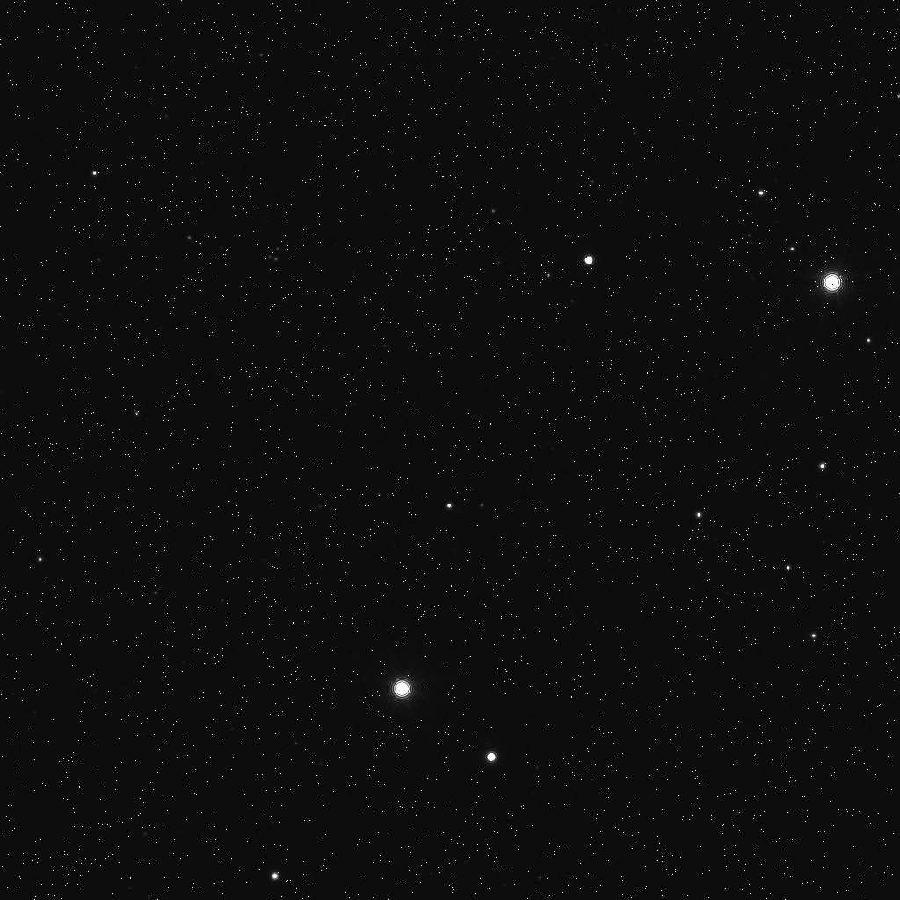
\includegraphics[width=0.24\textwidth]{Figures/Simulated_130_12.pdf} &
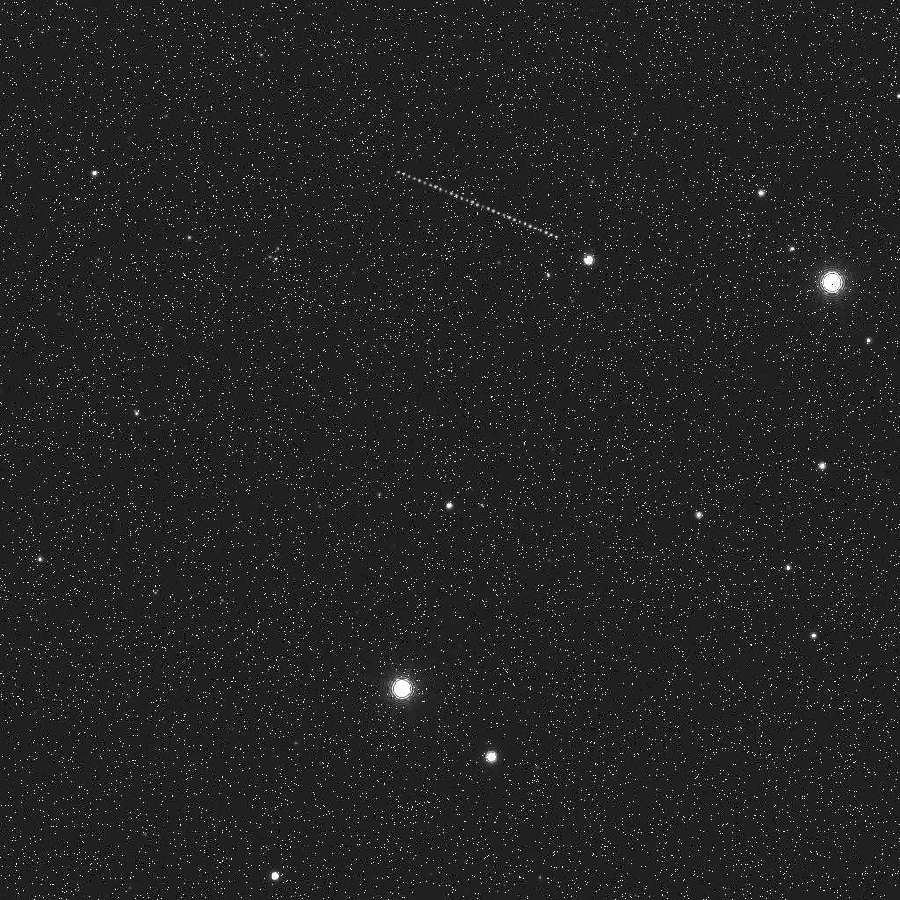
\includegraphics[width=0.24\textwidth]{Figures/TrueTrajectory_130.pdf} 
\end{array}$
\end{center}
\caption{Left: A simulated image generated by RCE. Right: 31 simulated MWIR images super-imposed in order to visualize the trajectory of the asteroid in a single image. The true trajectory can be seen as a faint line at the top center of the image}
\end{figure}

\begin{figure}[h]
\begin{center}$
\begin{array}{c@{\hspace{0.5em}}c@{\hspace{0.5em}}}
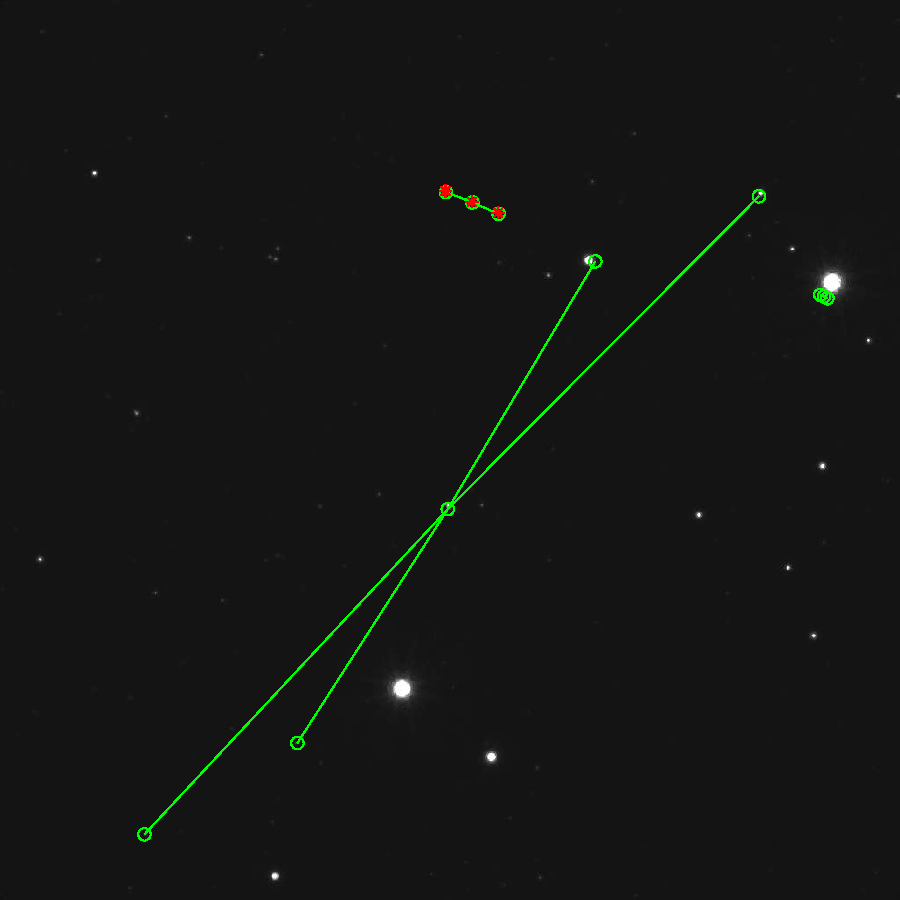
\includegraphics[width=0.24\textwidth]{Figures/Lines_011_016_021.pdf} &
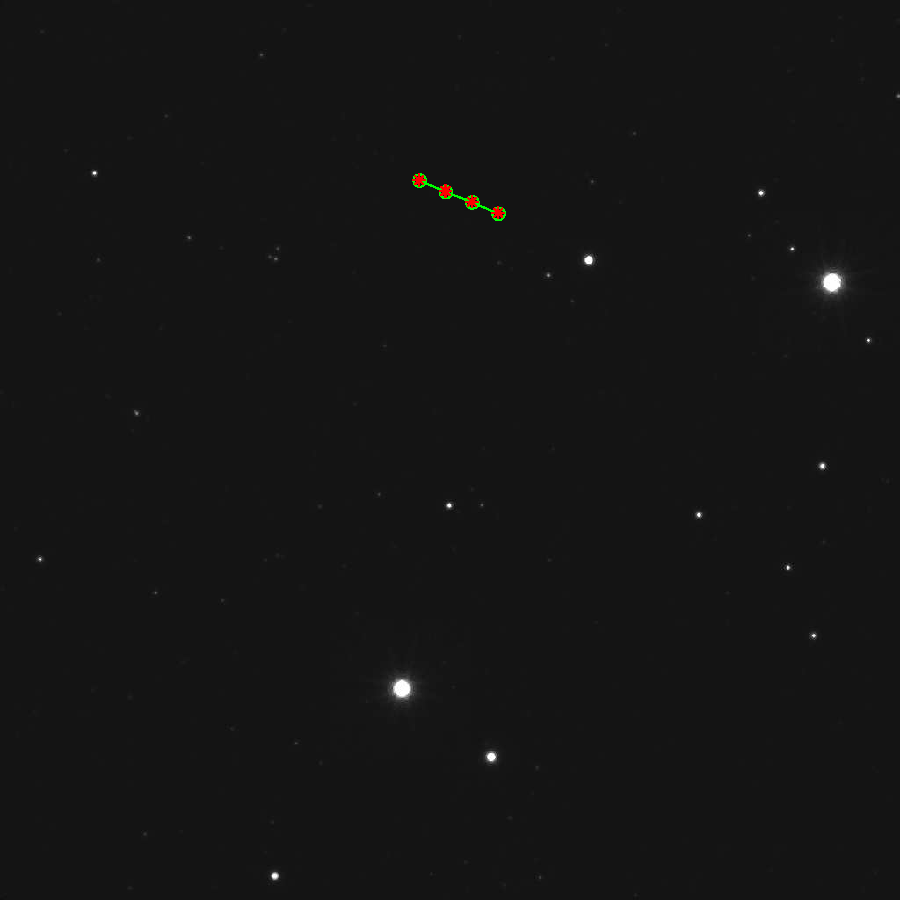
\includegraphics[width=0.24\textwidth]{Figures/Lines_011_016_021_026.pdf} 
\end{array}$
\end{center}
\caption{The trajectories found by the pipeline are shown in green. The true location of the asteroid is marked in red. Left: Trajectory Detection on a simulated triplet.  Right: Trajectory Detection on a quadruplet. Adding one more image to the triplet eliminates the false positives.}
\end{figure}

\begin{figure}[h]
\begin{center}$
\begin{array}{c@{\hspace{0.5em}}c@{\hspace{0.5em}}}
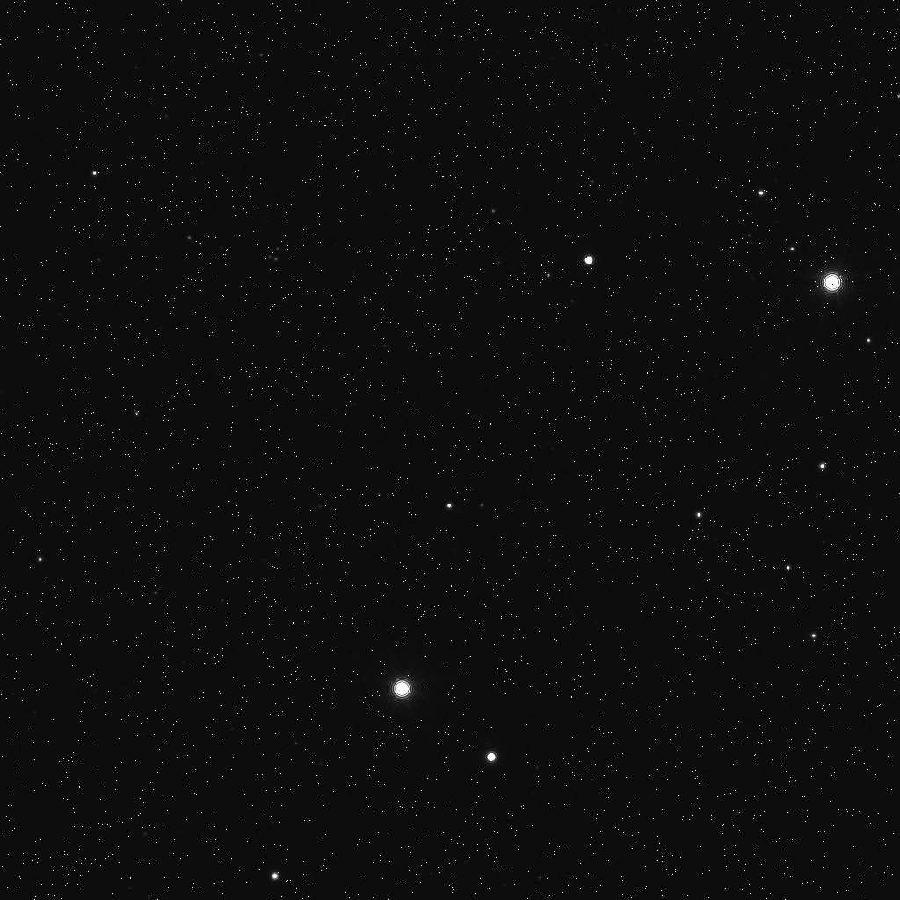
\includegraphics[width=0.24\textwidth]{Figures/Simulated_130_12.pdf} &
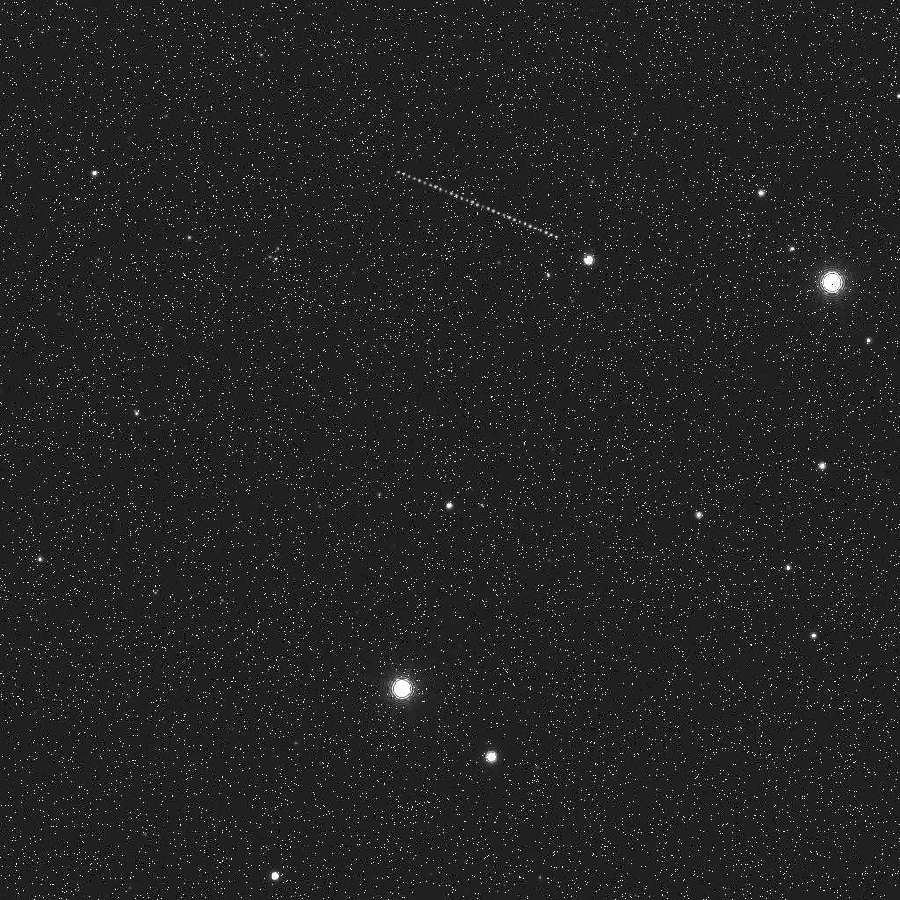
\includegraphics[width=0.24\textwidth]{Figures/TrueTrajectory_130.pdf} 
\end{array}$
\end{center}
\caption{Left:The number of detections at various stages of the pipeline for triplets of images. Right:  The number of detections at various stages of the pipeline for quadruplets of images.}
\end{figure}
 
\subsection{Real Imagery}
\label{ssec:real}

\subsubsection{NEAT}

The following figures show the results at all stages of the pipeline for one triplet of images of the 2002-CY46 asteroid obtained from the NEAT [24] survey.  
%\begin{figure*}
%\minipage{0.33\textwidth}
%  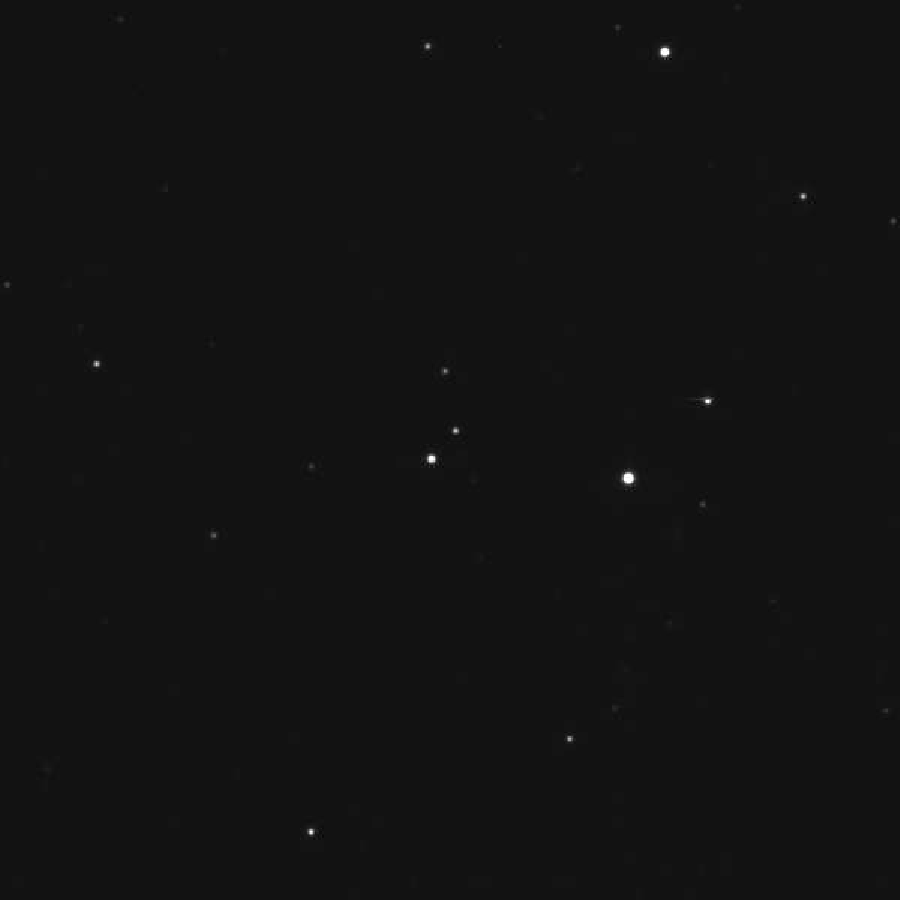
\includegraphics[width=\linewidth]{Figures/NEAT1.pdf}
%\endminipage\hfill
%\minipage{0.33\textwidth}
%  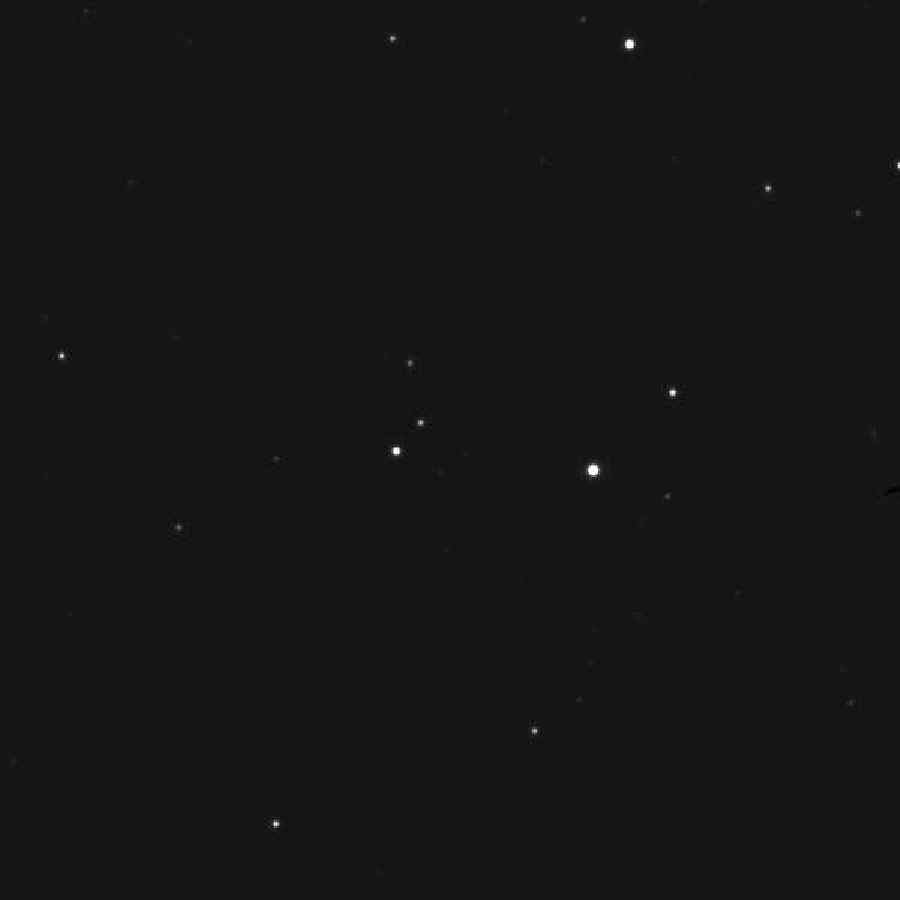
\includegraphics[width=\linewidth]{Figures/NEAT2.pdf}
%\endminipage\hfill
%\minipage{0.33\textwidth}
%  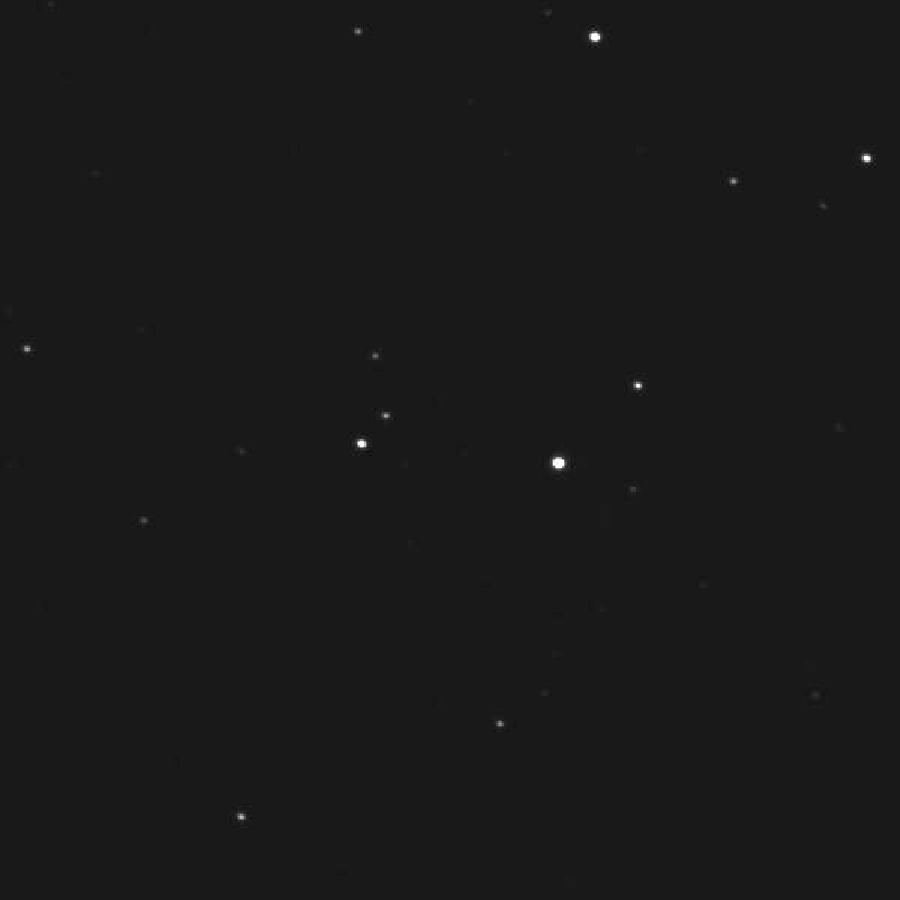
\includegraphics[width=\linewidth]{Figures/NEAT3.pdf}
%\endminipage
%\caption{2002 CY46 Triplet Near Earth Asteroid Tracking (NEAT) system archive}
%\label{fig:NEAT_Images}
%\end{figure*}

\newcommand{\imgWidth}{0.14\textwidth}
\begin{figure}[h]
\begin{center}$
\begin{array}{c@{\hspace{0.5em}}c@{\hspace{0.5em}}c}
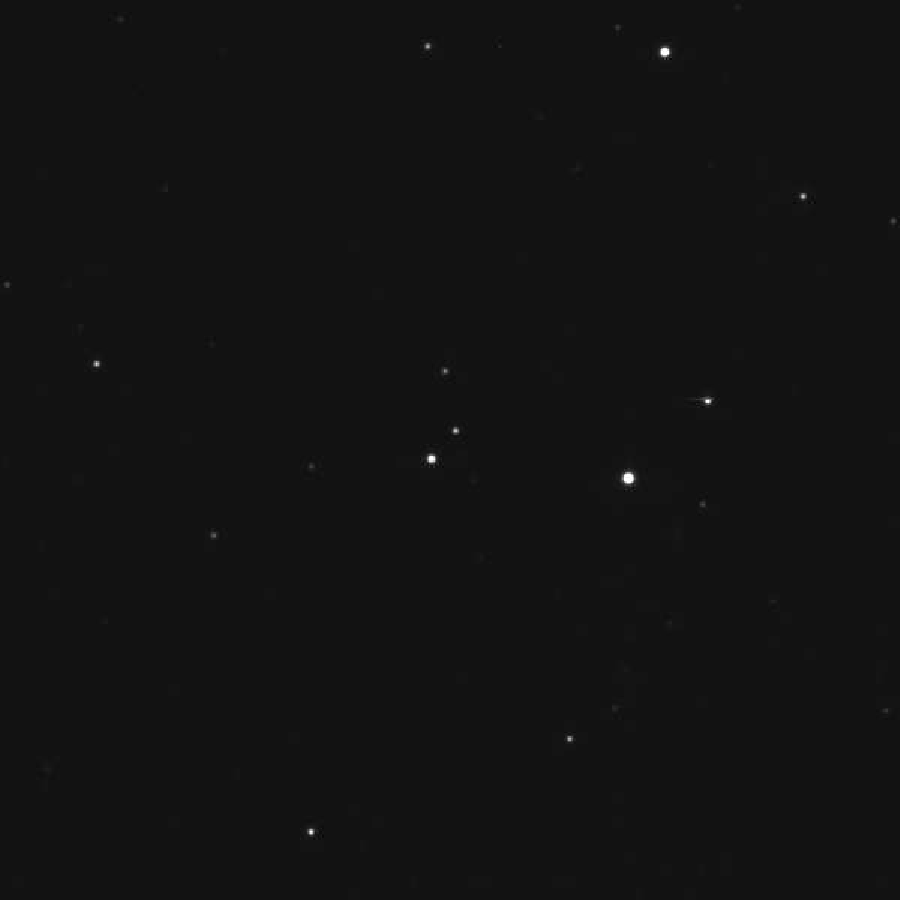
\includegraphics[width=\imgWidth]{Figures/NEAT1.pdf} &
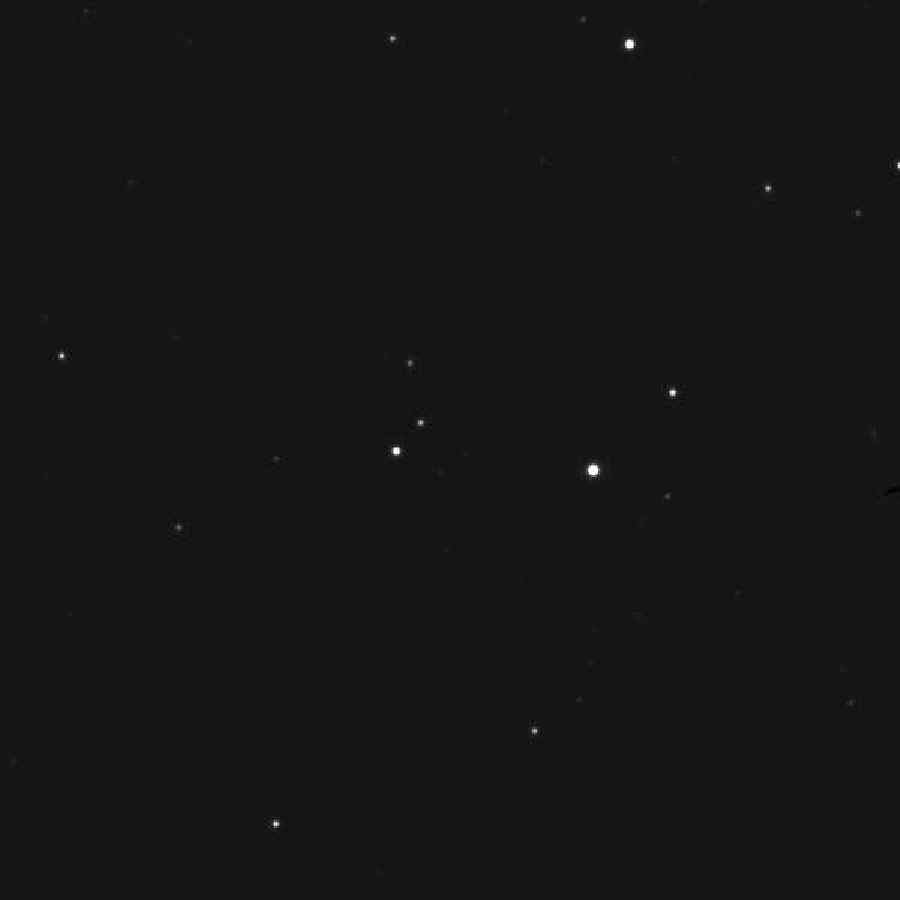
\includegraphics[width=\imgWidth]{Figures/NEAT2.pdf} &
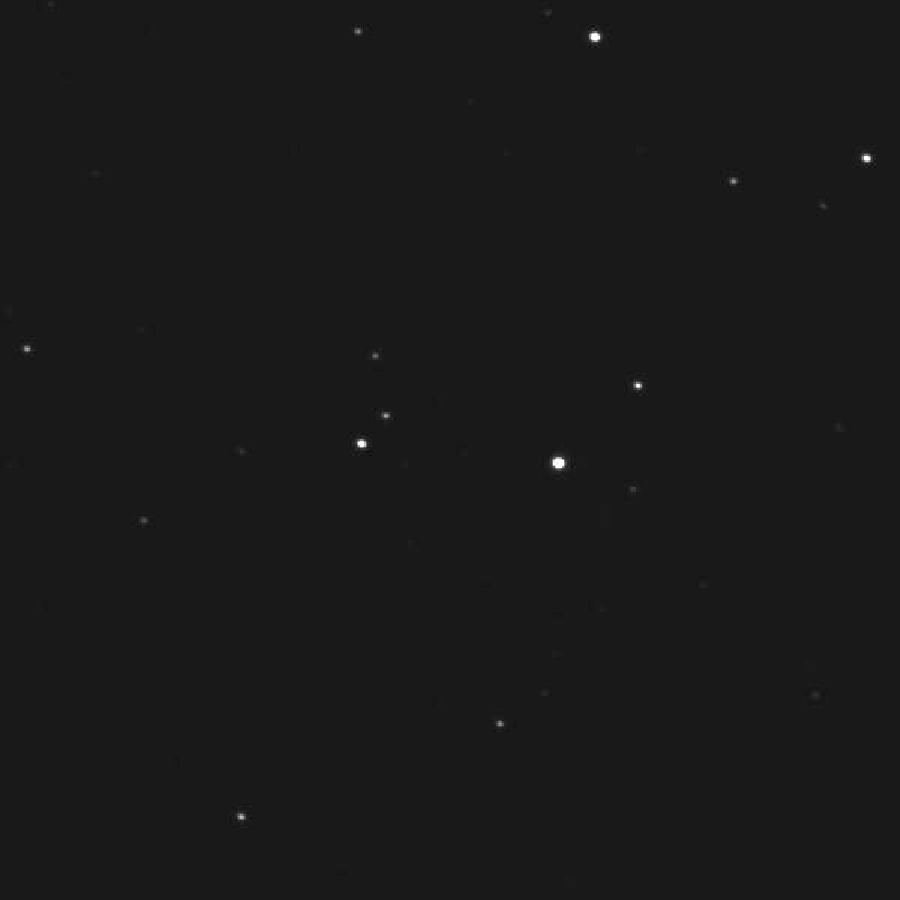
\includegraphics[width=\imgWidth]{Figures/NEAT3.pdf} \\
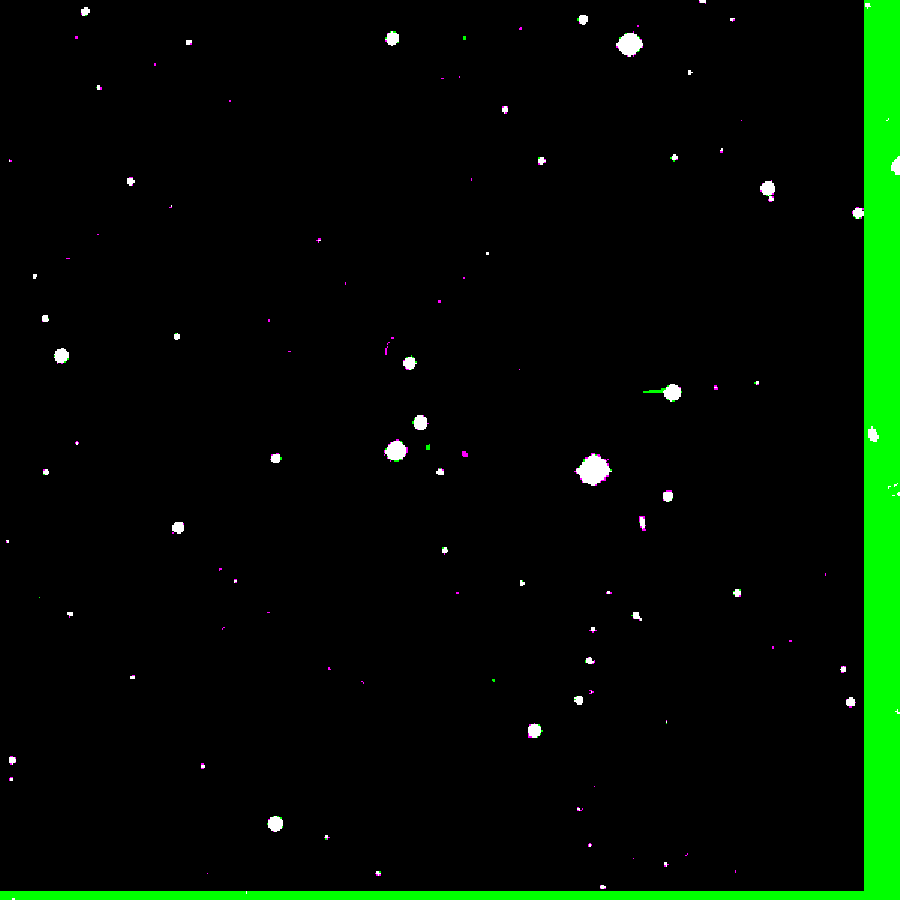
\includegraphics[width=\imgWidth]{Figures/NEATImageReg12.pdf} &
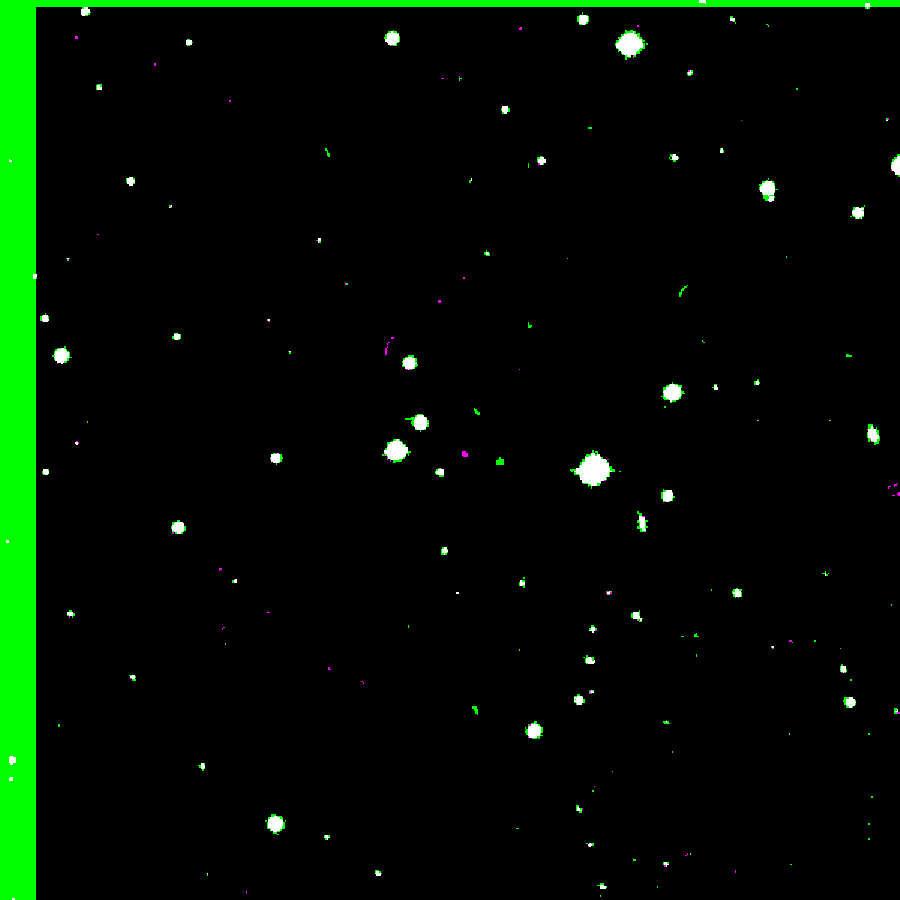
\includegraphics[width=\imgWidth]{Figures/NEATImageReg32.pdf} \\
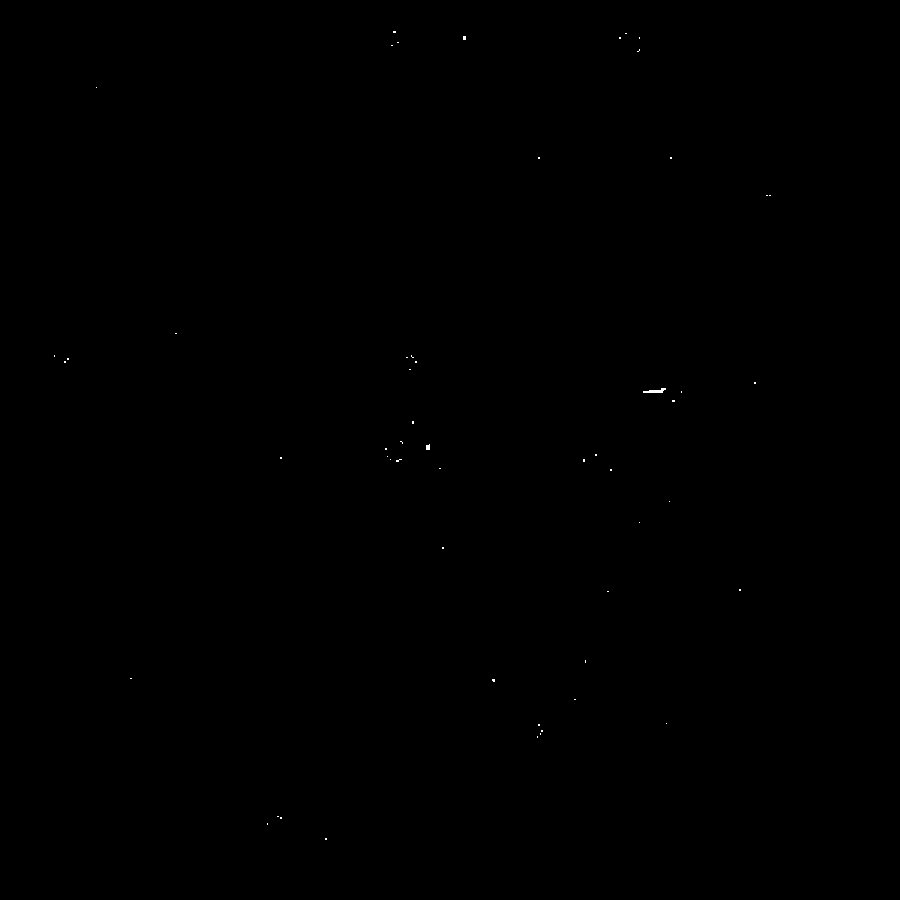
\includegraphics[width=\imgWidth]{Figures/NEATImageDiff1.pdf} &
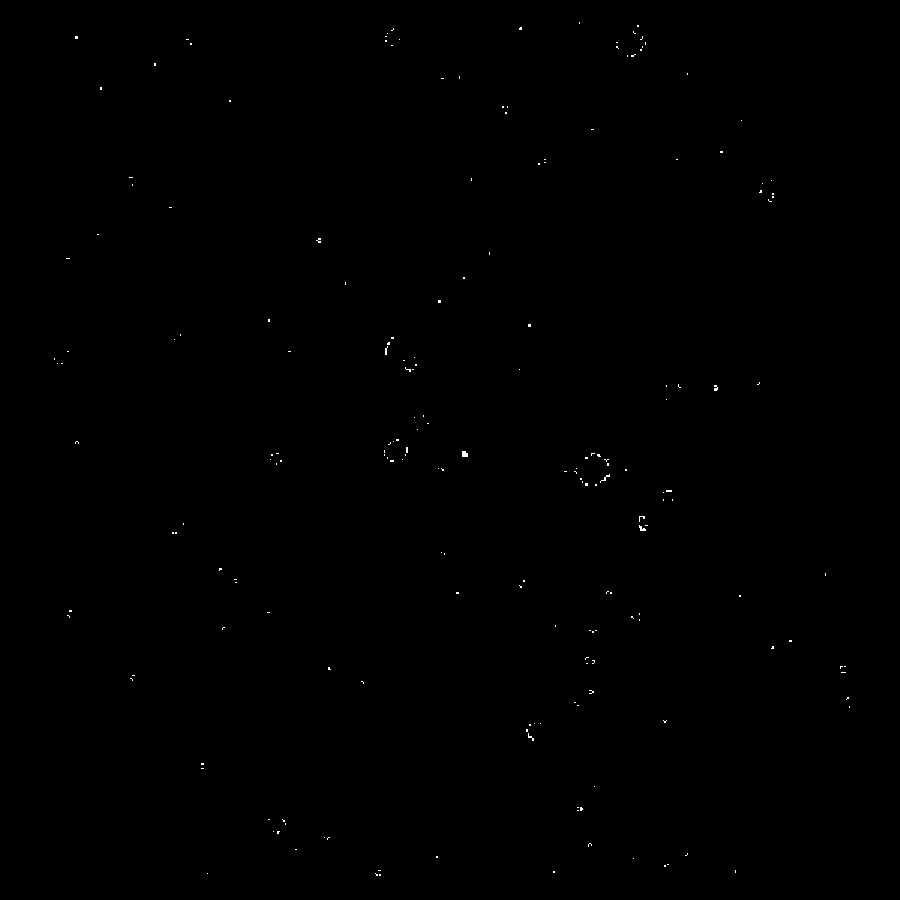
\includegraphics[width=\imgWidth]{Figures/NEATImageDiff2.pdf} &
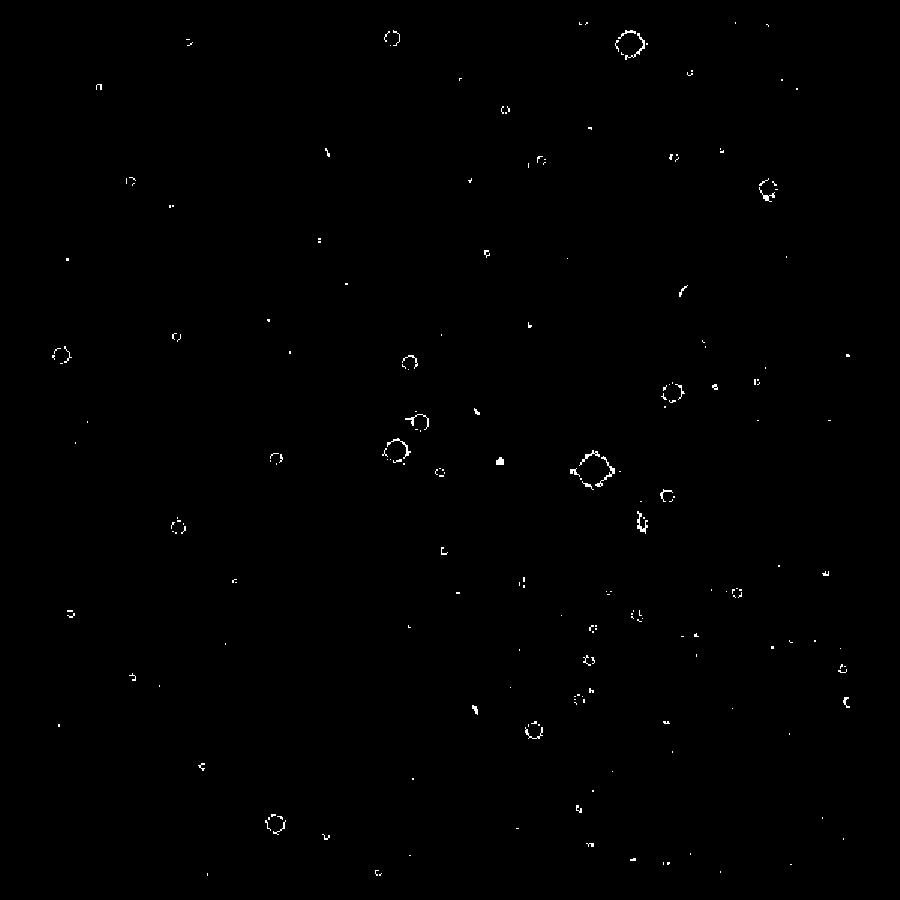
\includegraphics[width=\imgWidth]{Figures/NEATImageDiff3.pdf} \\
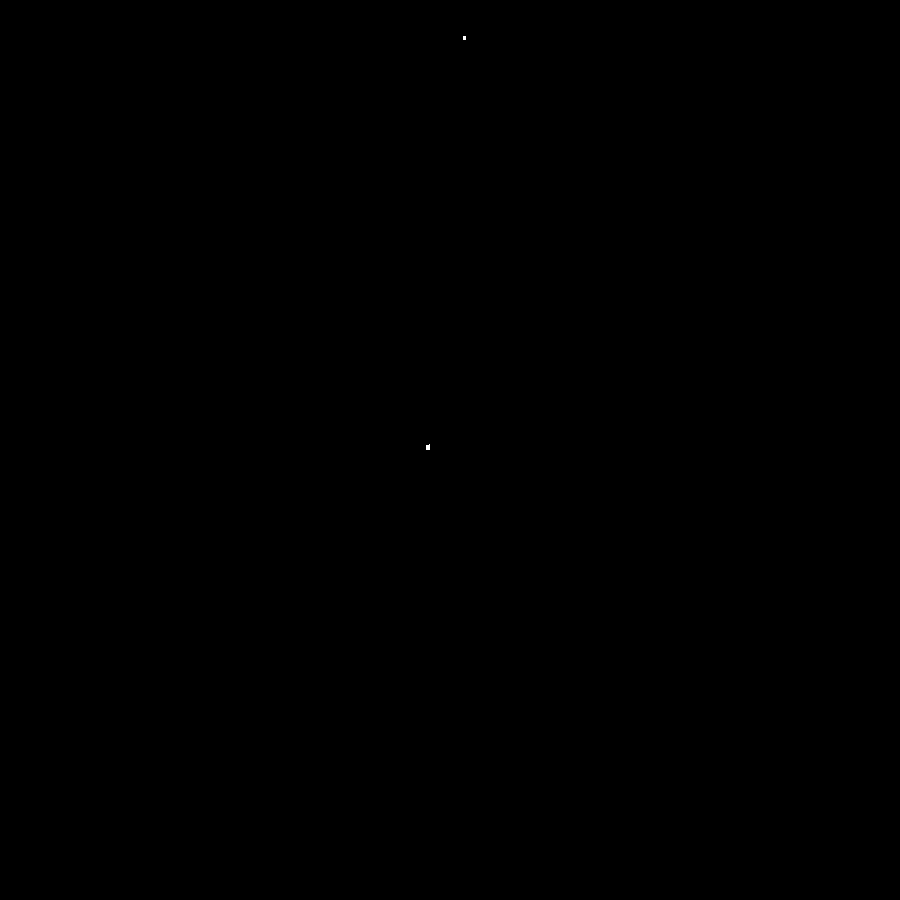
\includegraphics[width=\imgWidth]{Figures/NEATFilteredCentroids1.pdf} &
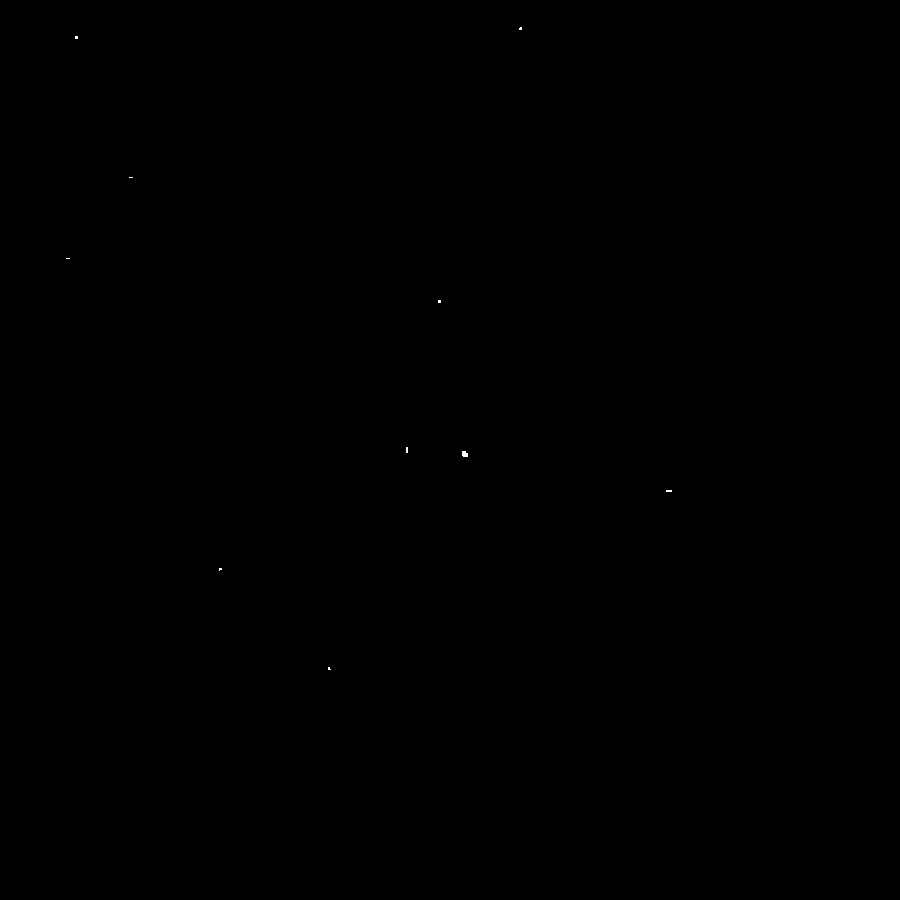
\includegraphics[width=\imgWidth]{Figures/NEATFilteredCentroids2.pdf} &
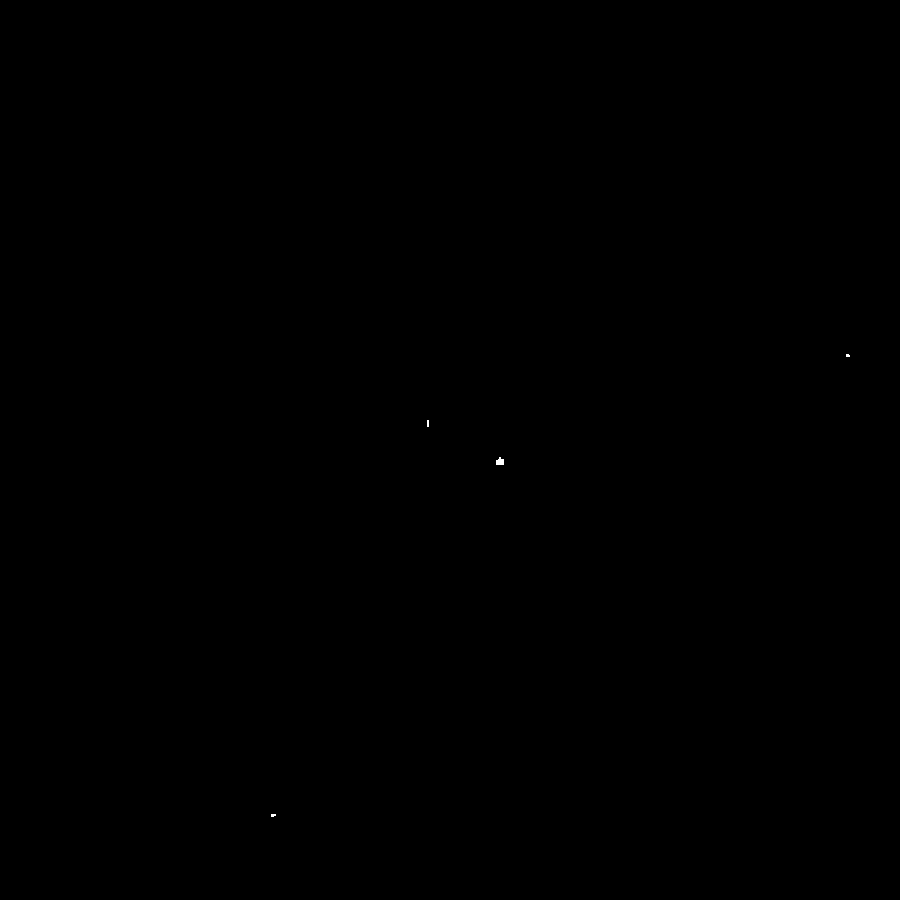
\includegraphics[width=\imgWidth]{Figures/NEATFilteredCentroids3.pdf}
\end{array}$
\end{center}
\caption{Option 1. Image Processing Pipeline results. 
First row: 2002 CY46 Triplet images taken 10 minutes apart. Near Earth Asteroid Tracking (NEAT) system archive. 
Second row: Image Registration results for the CY46 Triplet.  Left: Image-1 registered to Image-2. Right: Image-3 registered to Image-2.
Third row: Image Differencing results for the CY46 Triplet. (Artifacts such as crater-like formations are seen in the difference images above. This is the result of some celestial bodies being over-exposed.) 
Fourth row: Image Differencing results for the CY46 Triplet. Filtered centroids in each image of the sequence.)}
\end{figure}

\newcommand{\imgWidthMedium}{0.23\textwidth}
\begin{figure*}[h]
\begin{center}$
\begin{array}{c@{\hspace{.5em}}c@{\hspace{0.5em}}c@{\hspace{0.5em}}c}
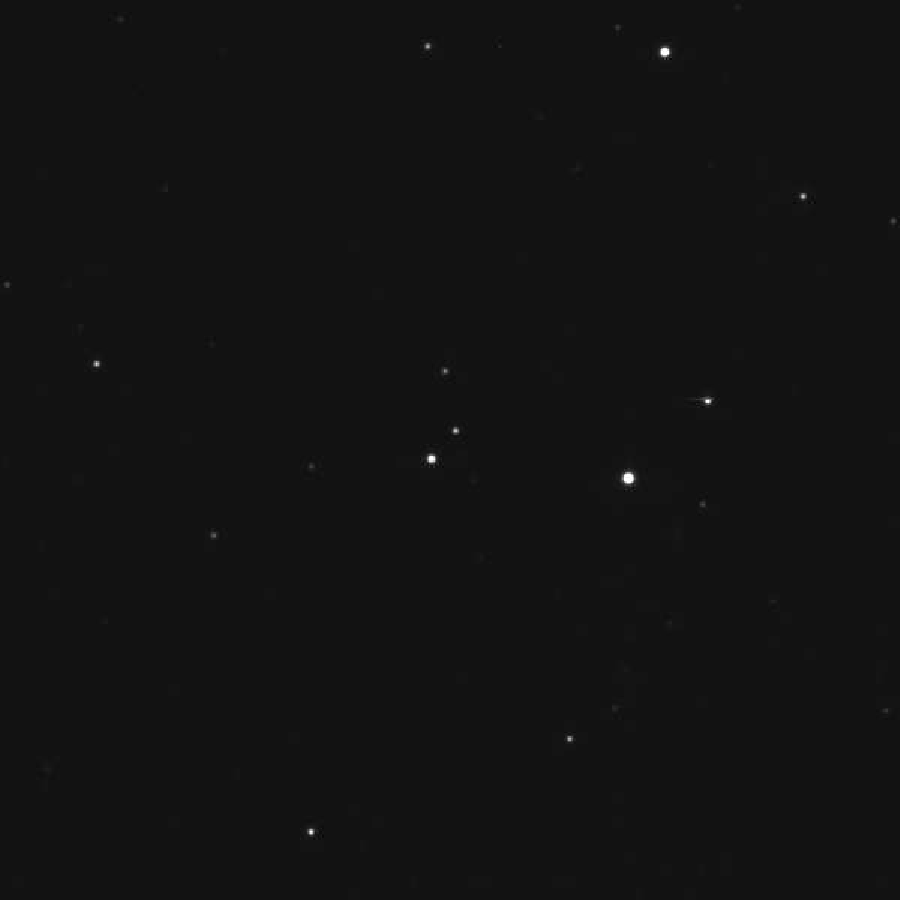
\includegraphics[width=\imgWidthMedium]{Figures/NEAT1.pdf} &
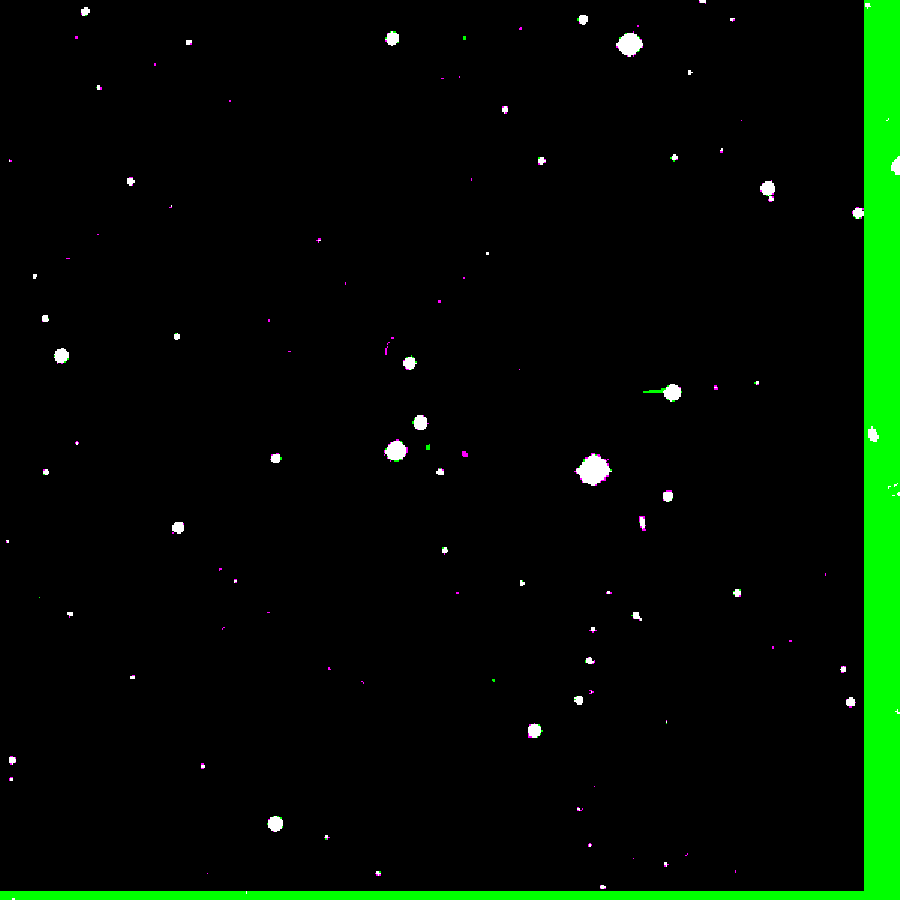
\includegraphics[width=\imgWidthMedium]{Figures/NEATImageReg12.pdf} &
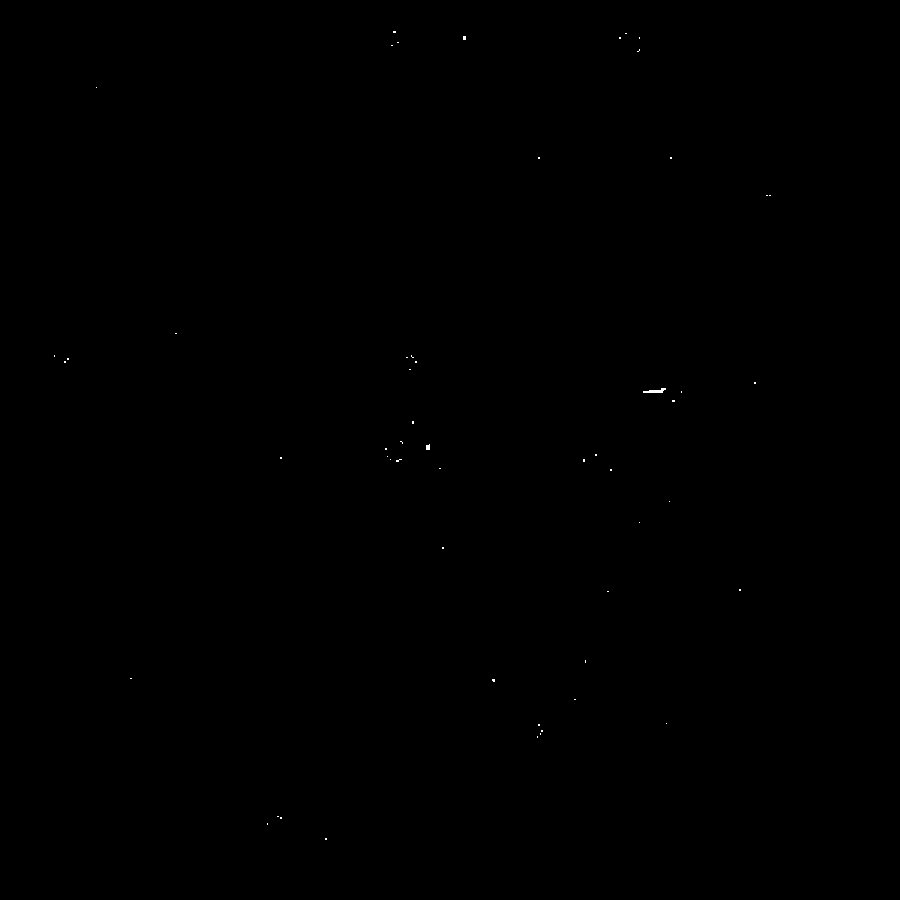
\includegraphics[width=\imgWidthMedium]{Figures/NEATImageDiff1.pdf} &
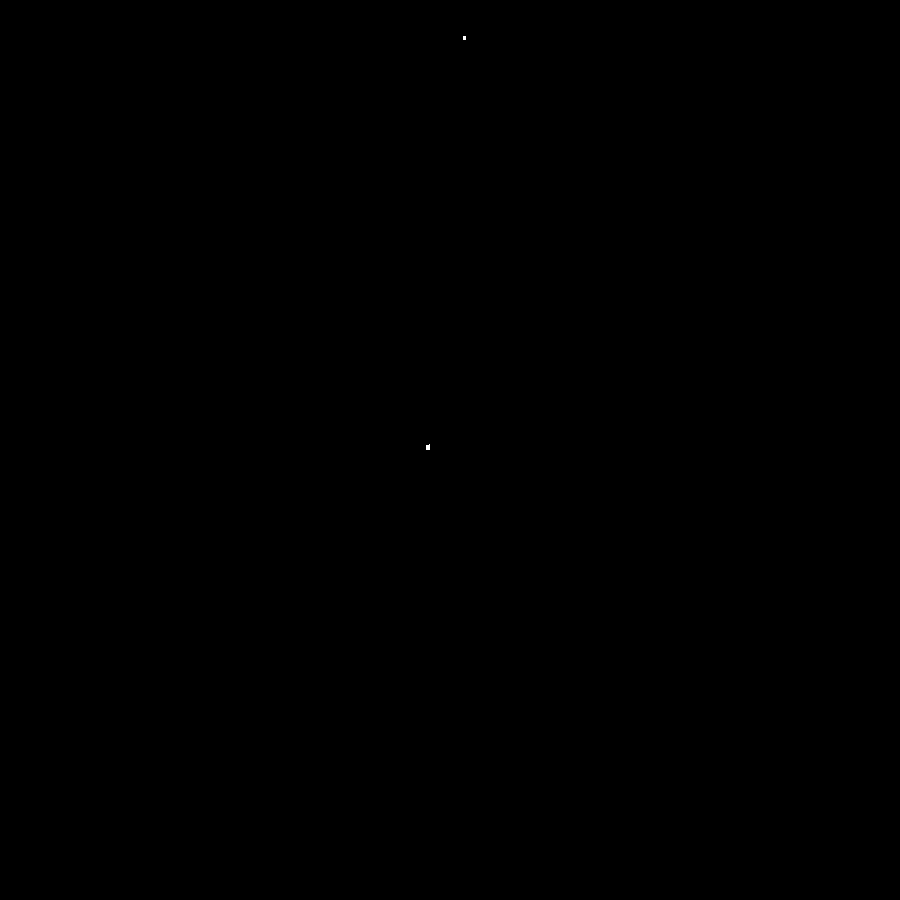
\includegraphics[width=\imgWidthMedium]{Figures/NEATFilteredCentroids1.pdf} \\
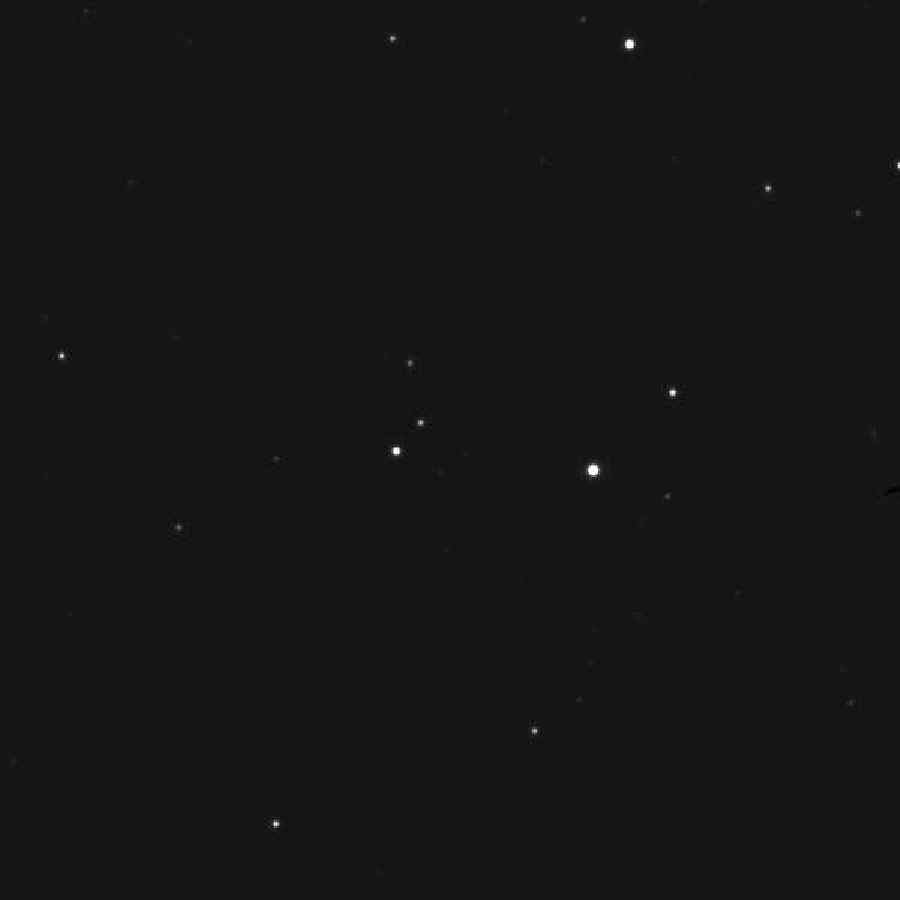
\includegraphics[width=\imgWidthMedium]{Figures/NEAT2.pdf} &
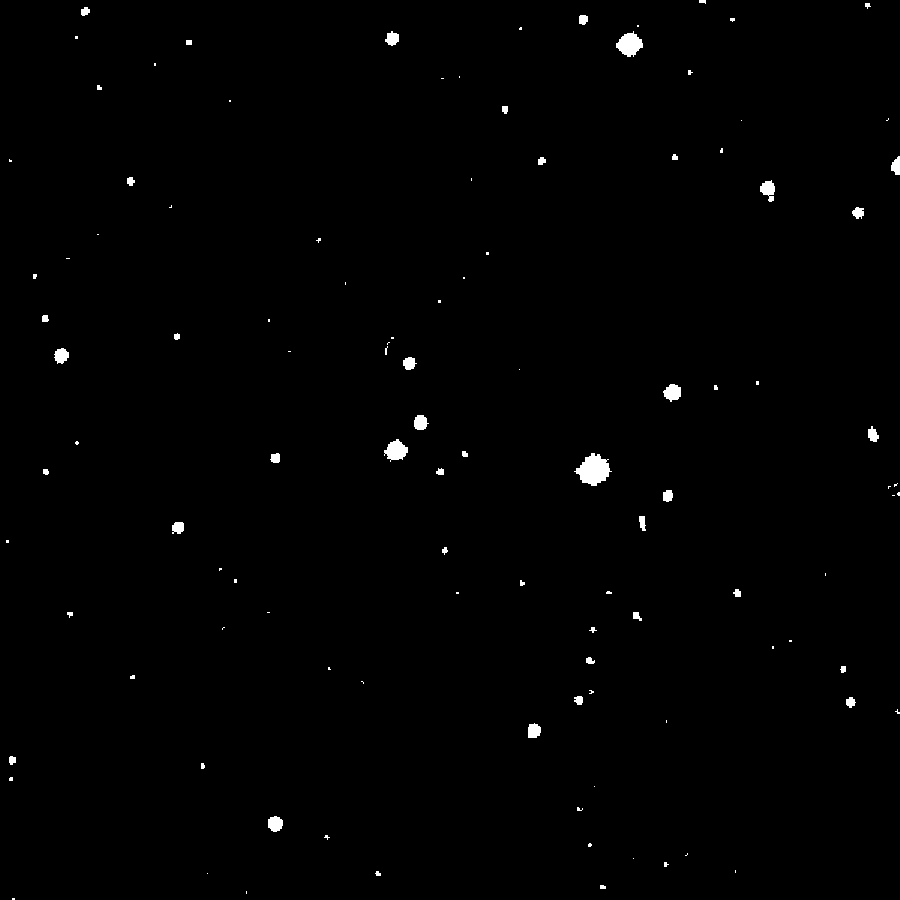
\includegraphics[width=\imgWidthMedium]{Figures/NEATImageReg22.pdf} &
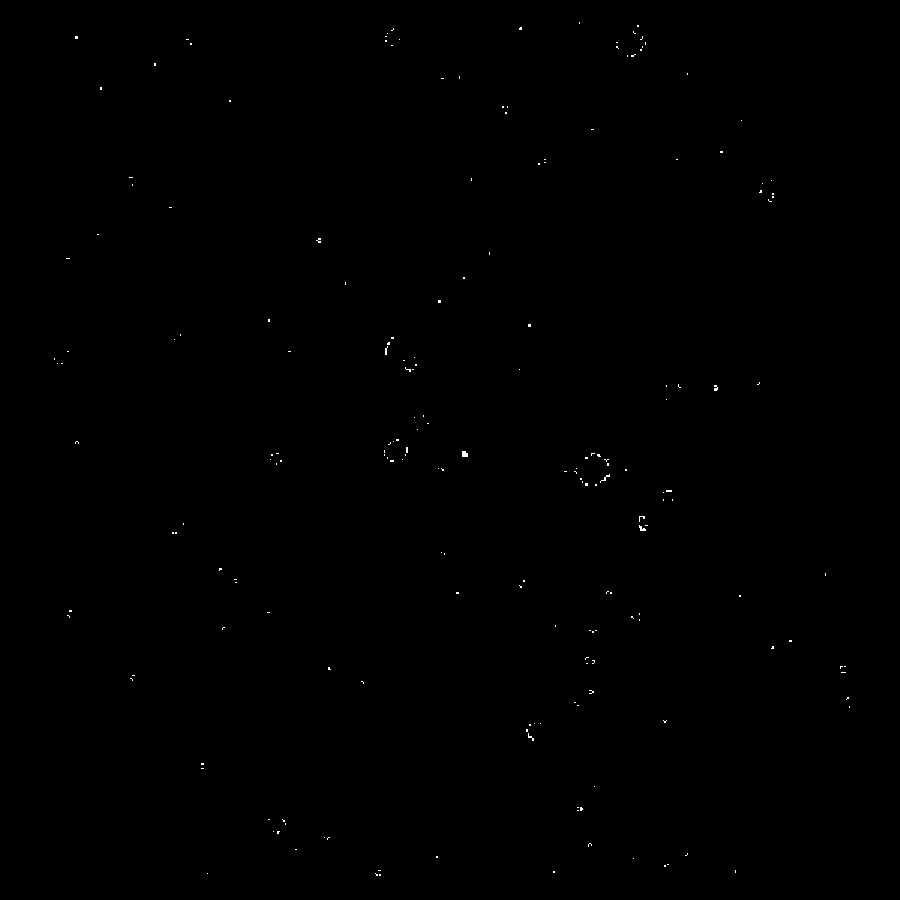
\includegraphics[width=\imgWidthMedium]{Figures/NEATImageDiff2.pdf} &
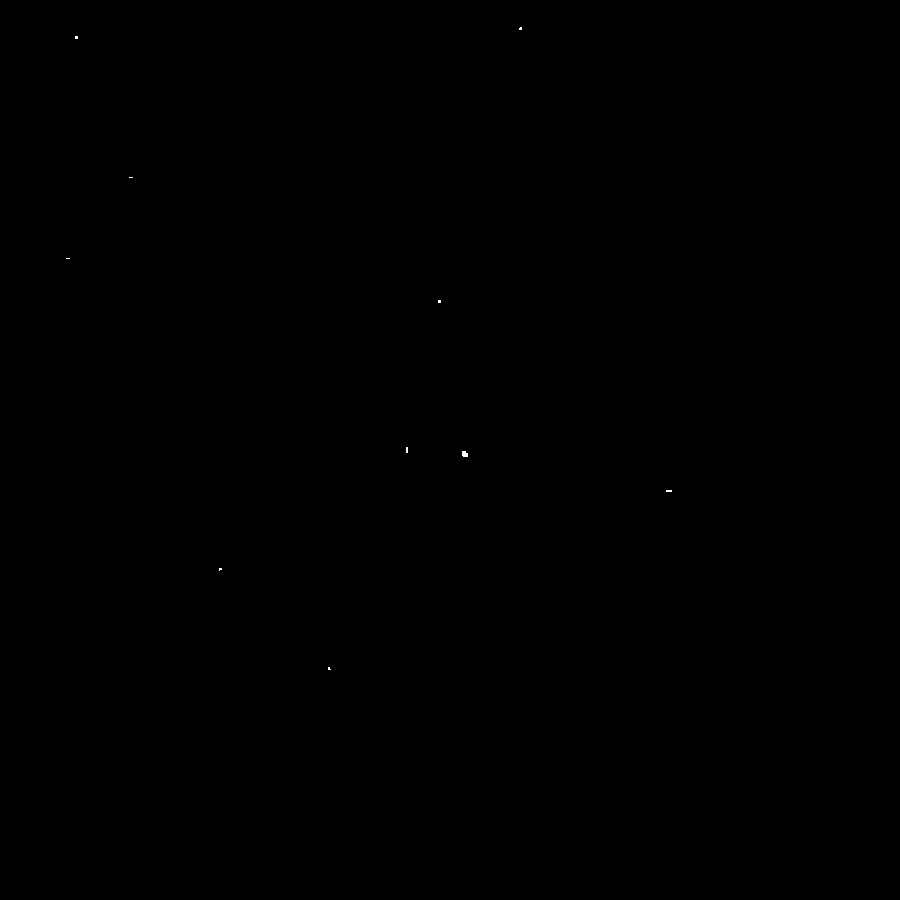
\includegraphics[width=\imgWidthMedium]{Figures/NEATFilteredCentroids2.pdf} \\
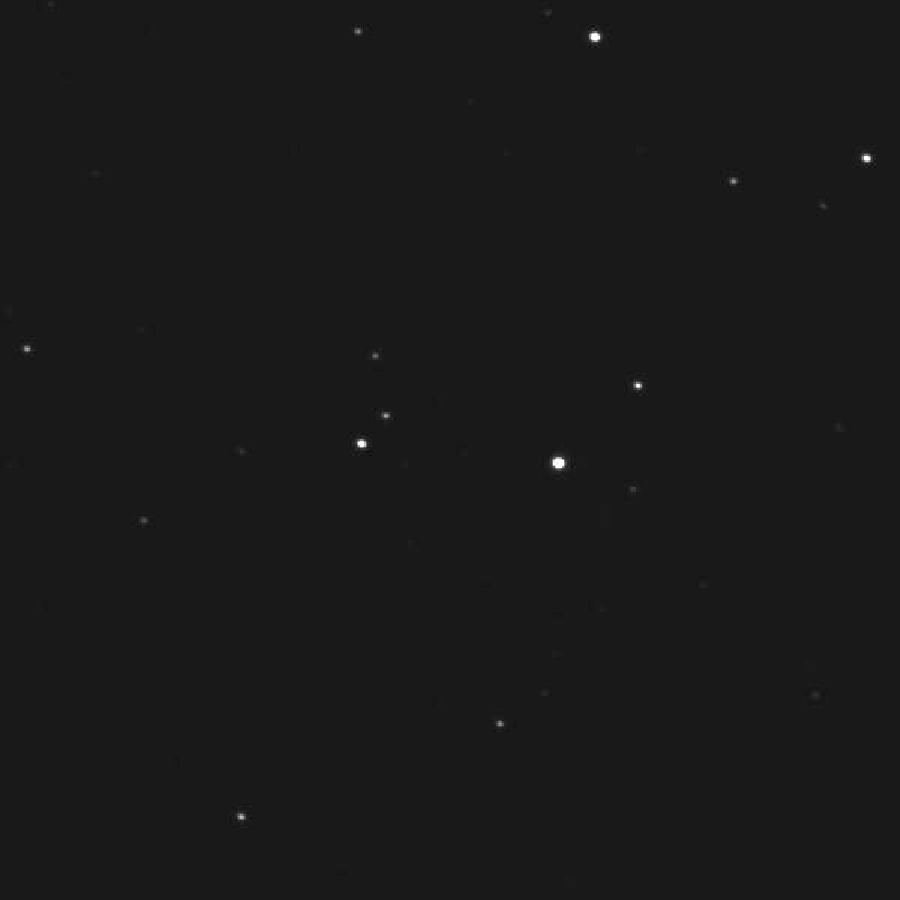
\includegraphics[width=\imgWidthMedium]{Figures/NEAT3.pdf} &
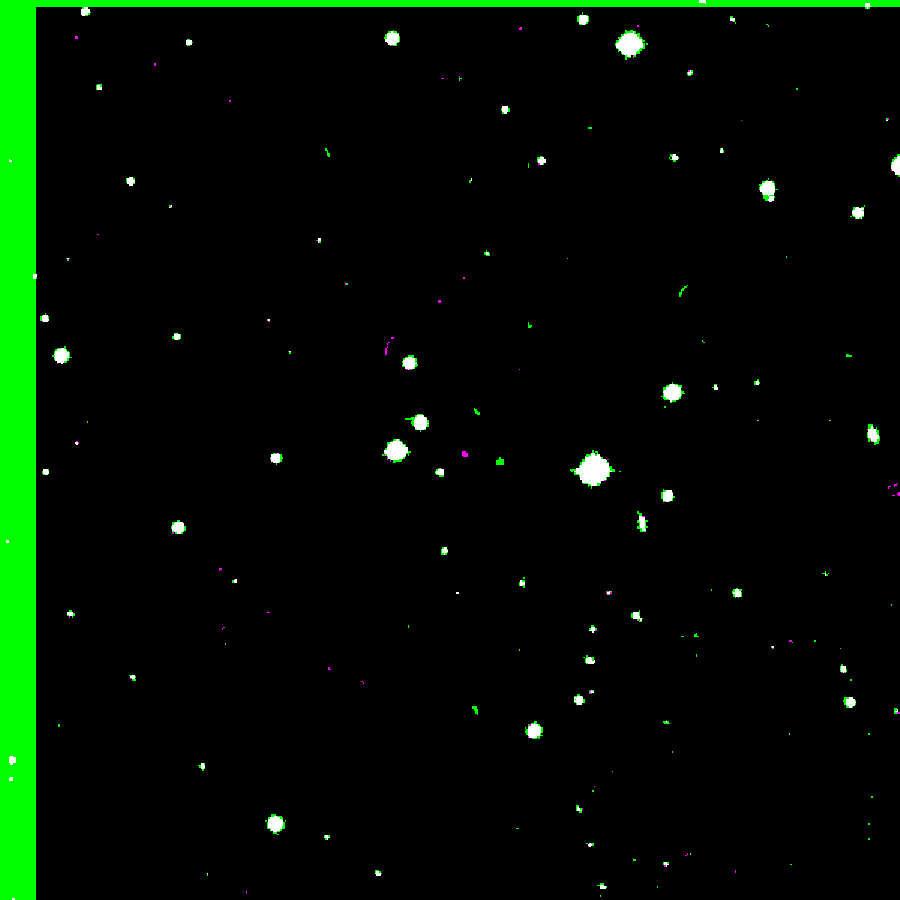
\includegraphics[width=\imgWidthMedium]{Figures/NEATImageReg32.pdf} &
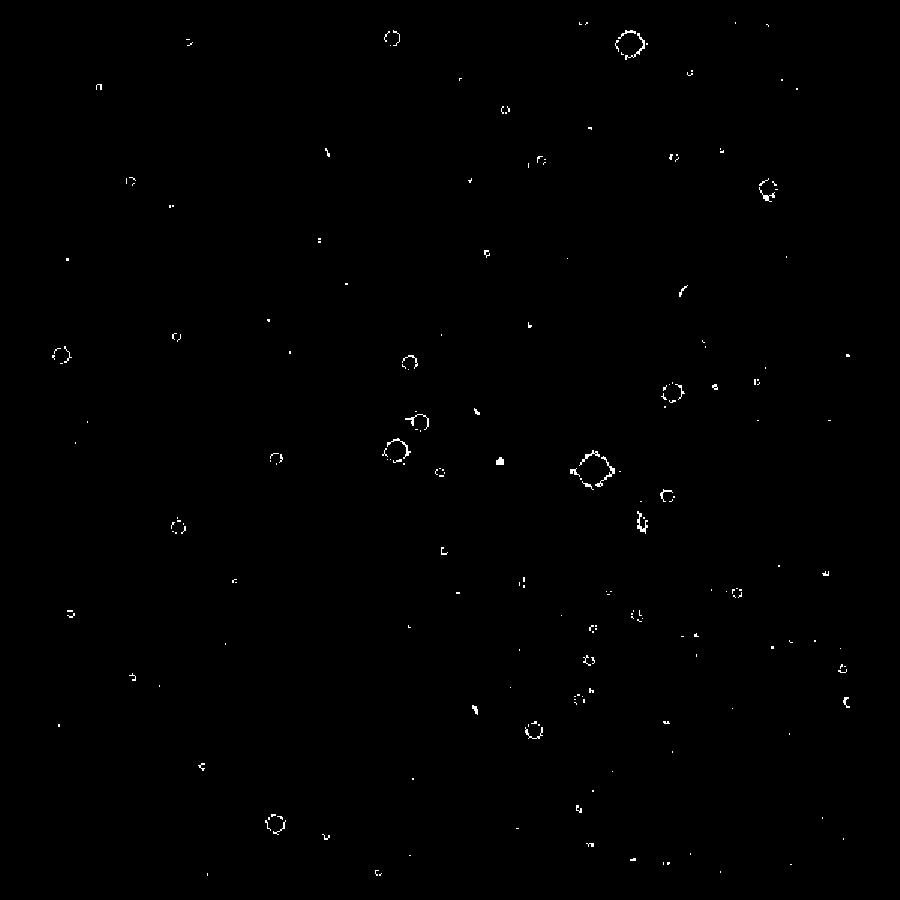
\includegraphics[width=\imgWidthMedium]{Figures/NEATImageDiff3.pdf} &
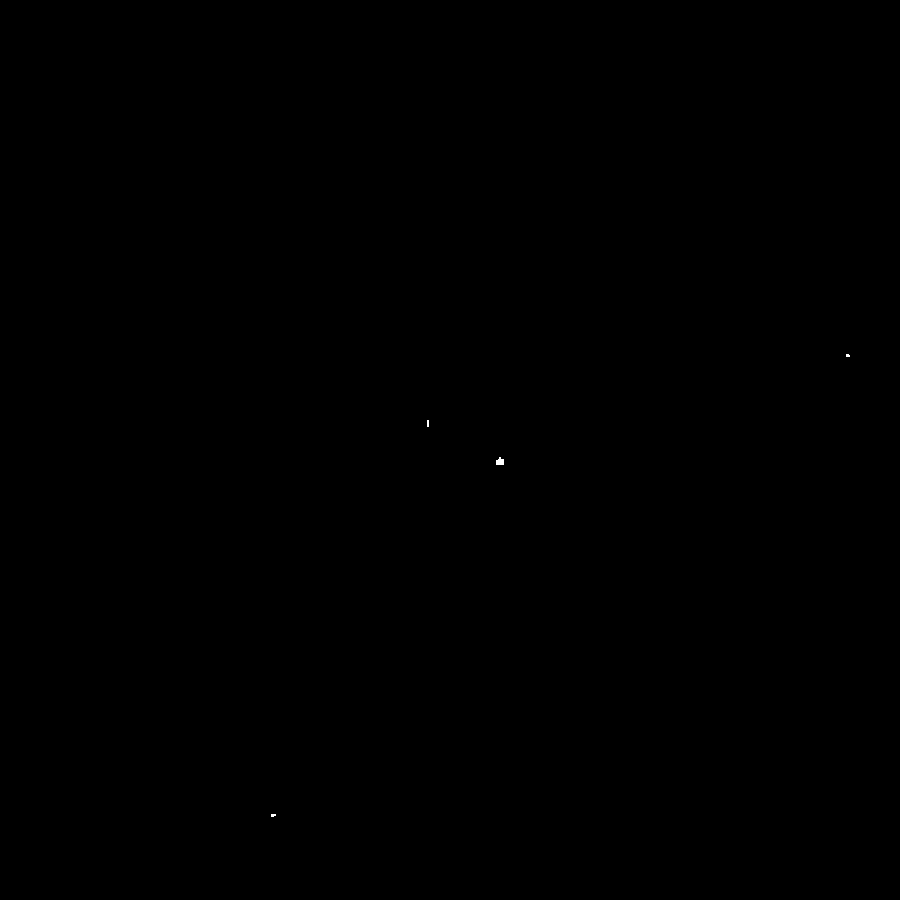
\includegraphics[width=\imgWidthMedium]{Figures/NEATFilteredCentroids3.pdf} 
\end{array}$
\end{center}
\caption[caption]{Option 2. Image Processing Pipeline results. \\\hspace{\textwidth} First column: 2002 CY46 Triplet images taken 10 minutes apart. Near Earth Asteroid Tracking (NEAT) system archive. \\\hspace{\textwidth} Second Column: Image Registration results for the CY46 Triplet.  Top: Image-1 registered to Image-2. Bottom: Image-3 registered to Image-2. \\\hspace{\textwidth} Third Column: Image Differencing results for the CY46 Triplet. (Artifacts such as crater-like formations are seen in the difference images above. This is the result of some celestial bodies being over-exposed.) \\\hspace{\textwidth} Fourth Column: Image Differencing results for the CY46 Triplet. Filtered centroids in each image of the sequence.)}
\end{figure*}

\begin{figure*}[h]
\begin{center}$
\begin{array}{ccc}
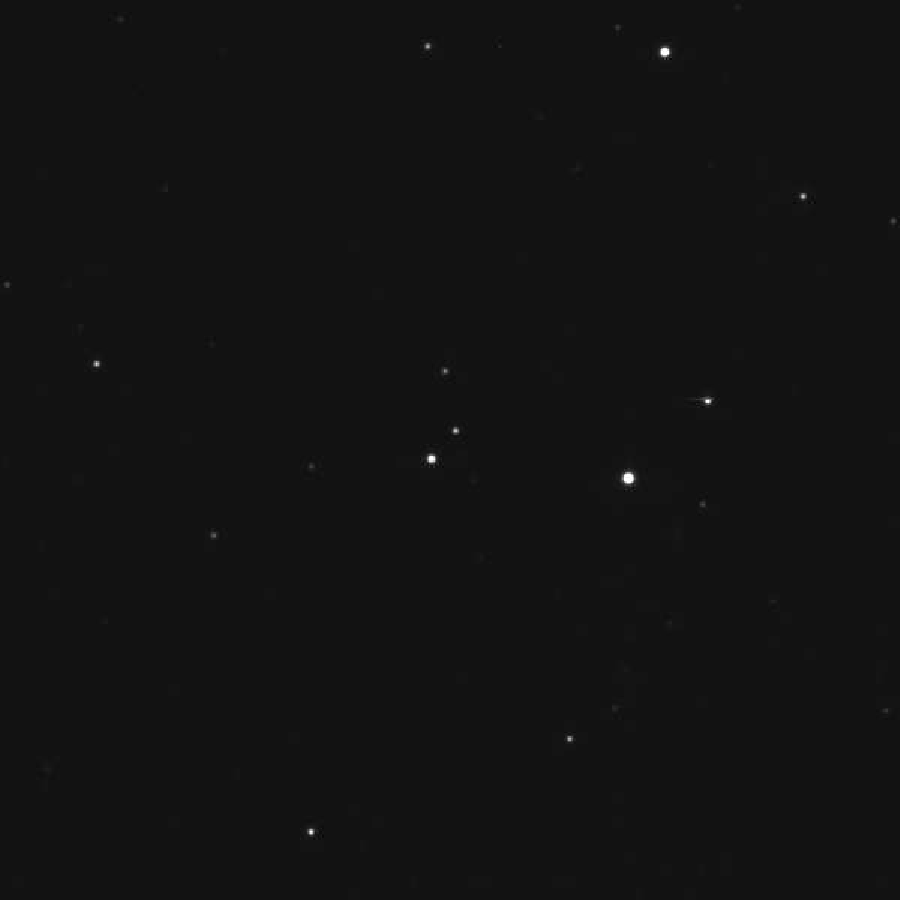
\includegraphics[width=0.33\textwidth]{Figures/NEAT1.pdf} &
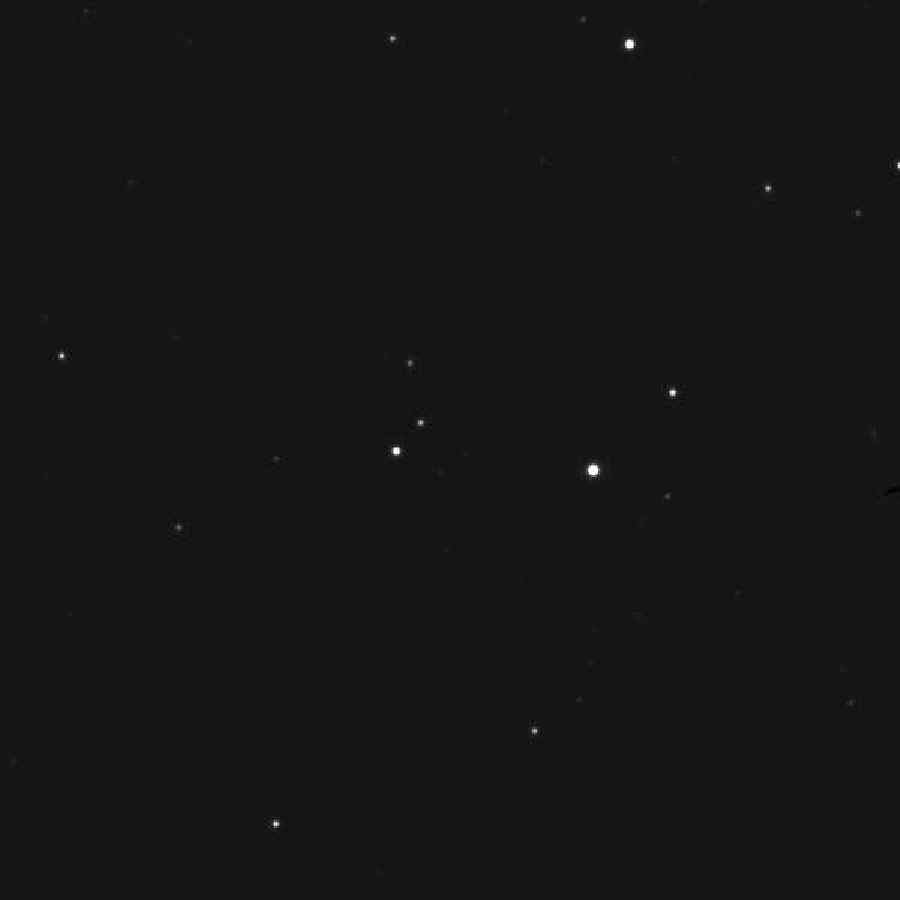
\includegraphics[width=0.33\textwidth]{Figures/NEAT2.pdf} &
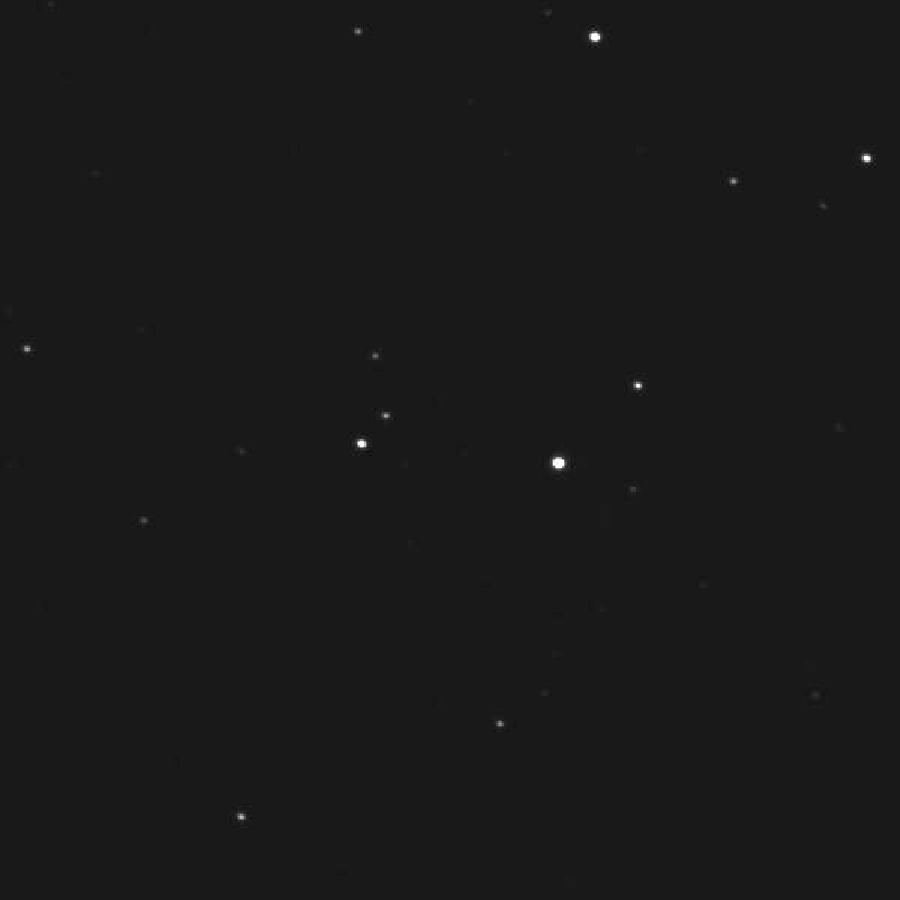
\includegraphics[width=0.33\textwidth]{Figures/NEAT3.pdf} \\
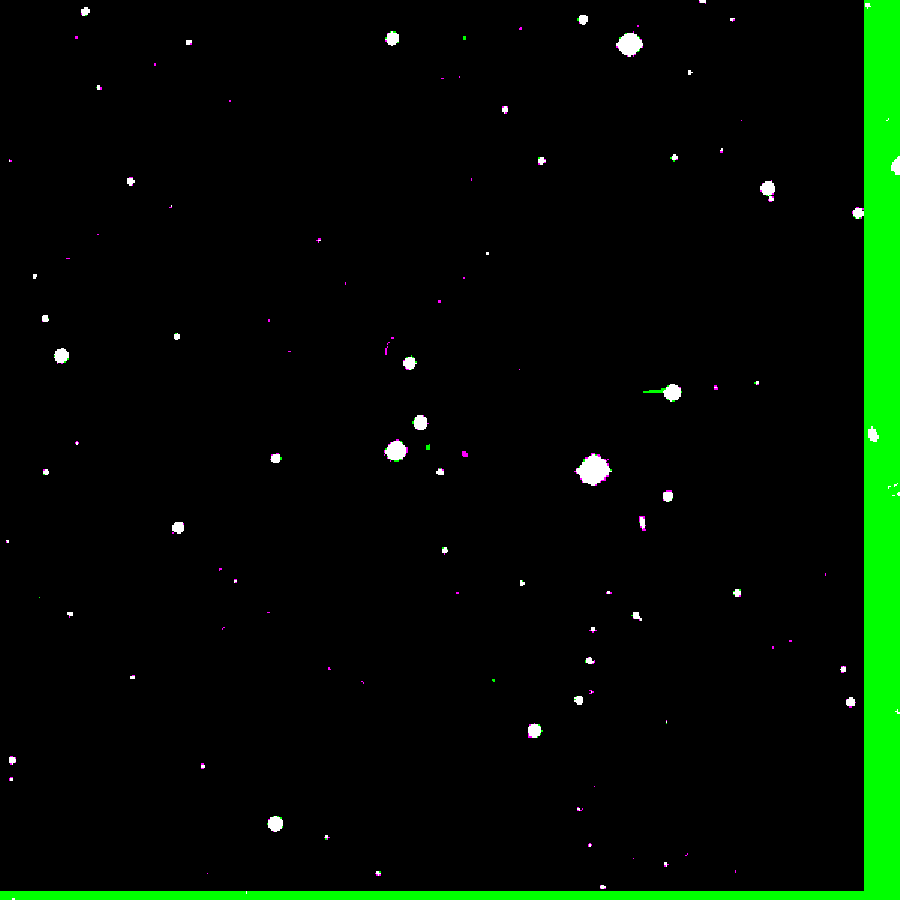
\includegraphics[width=0.33\textwidth]{Figures/NEATImageReg12.pdf} &
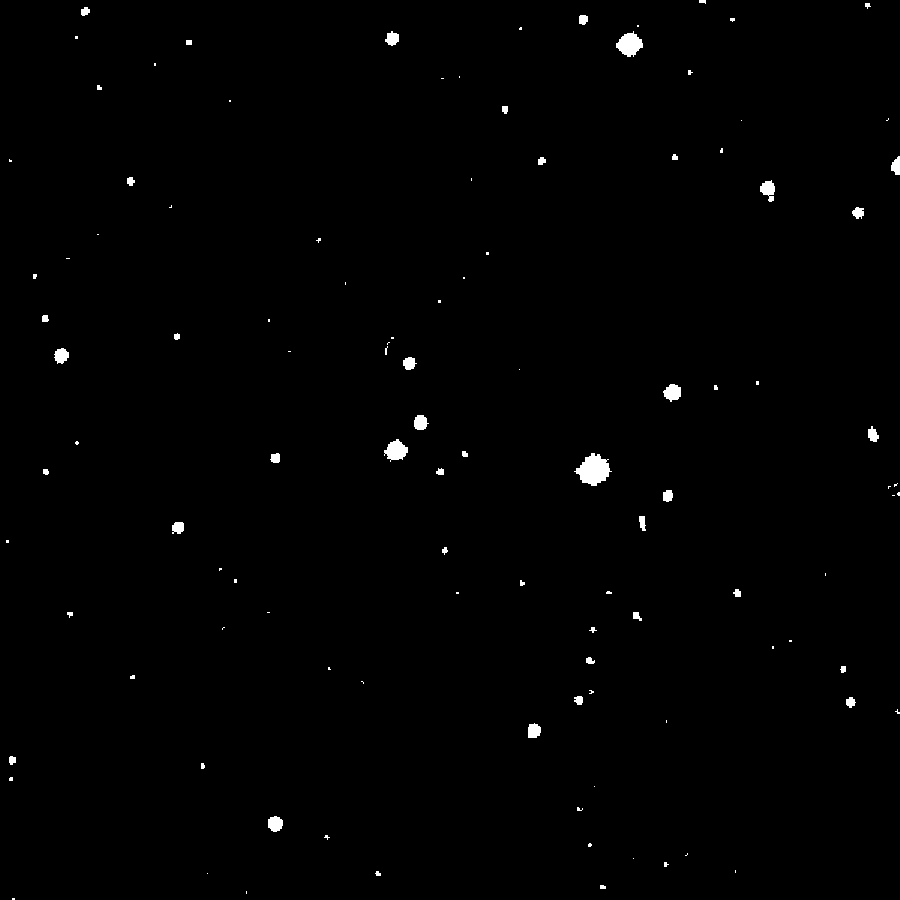
\includegraphics[width=0.33\textwidth]{Figures/NEATImageReg22.pdf} &
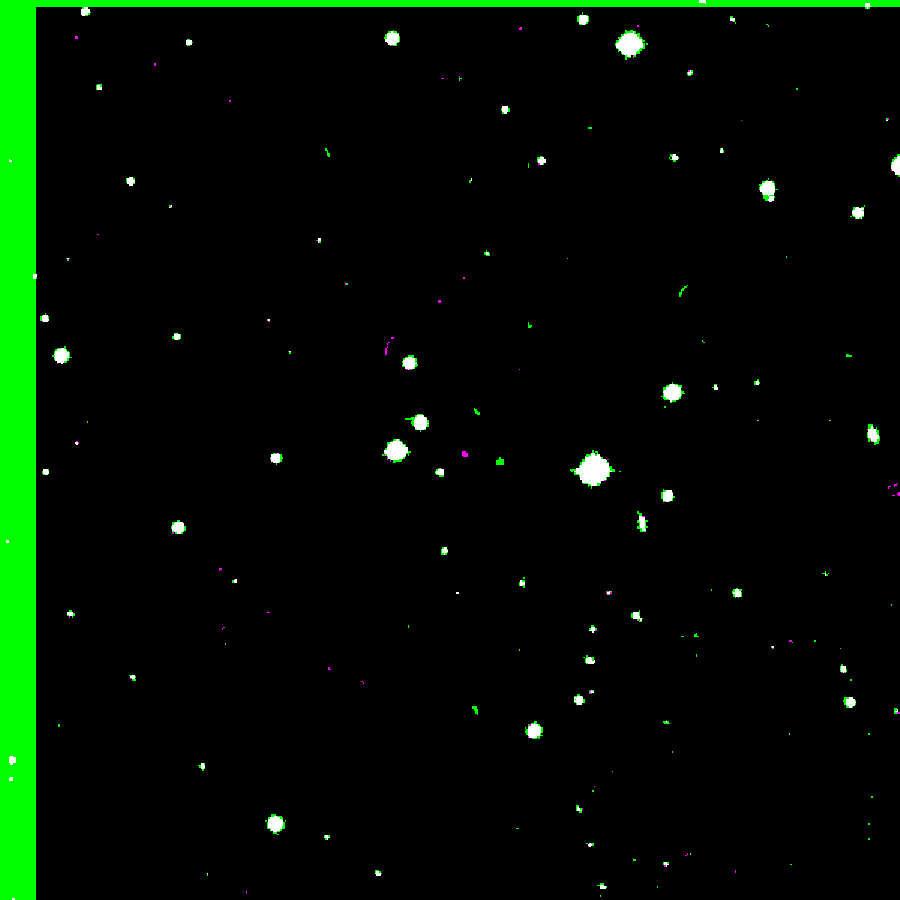
\includegraphics[width=0.33\textwidth]{Figures/NEATImageReg32.pdf} \\
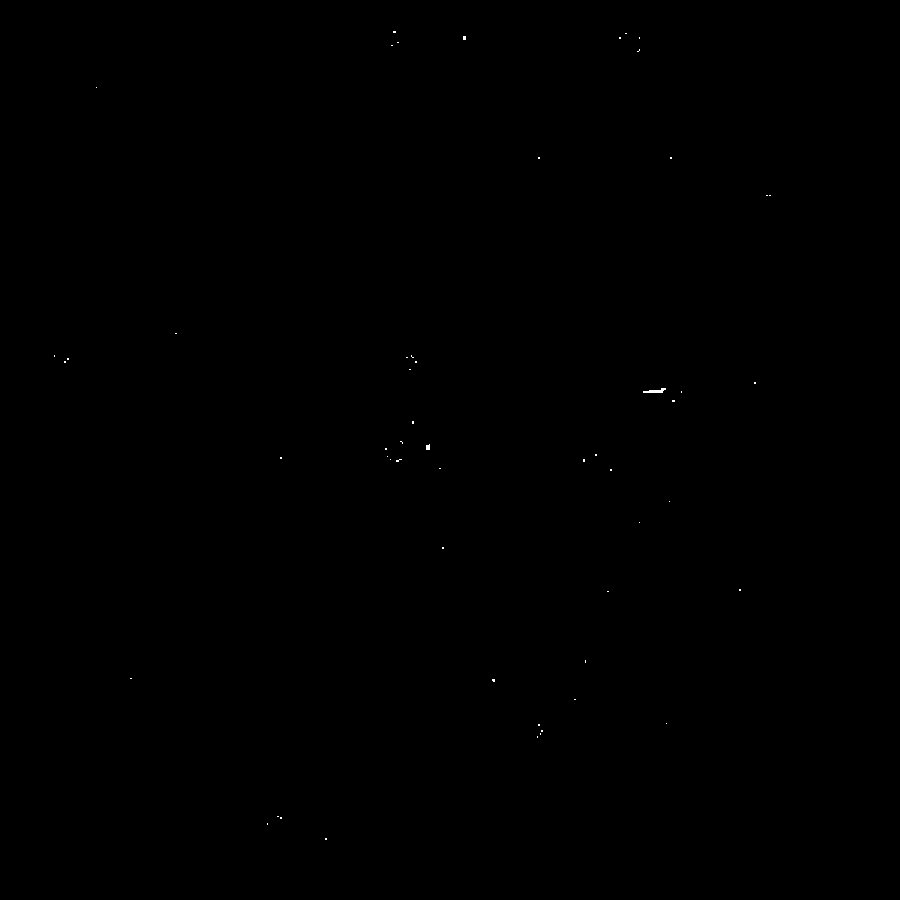
\includegraphics[width=0.33\textwidth]{Figures/NEATImageDiff1.pdf} &
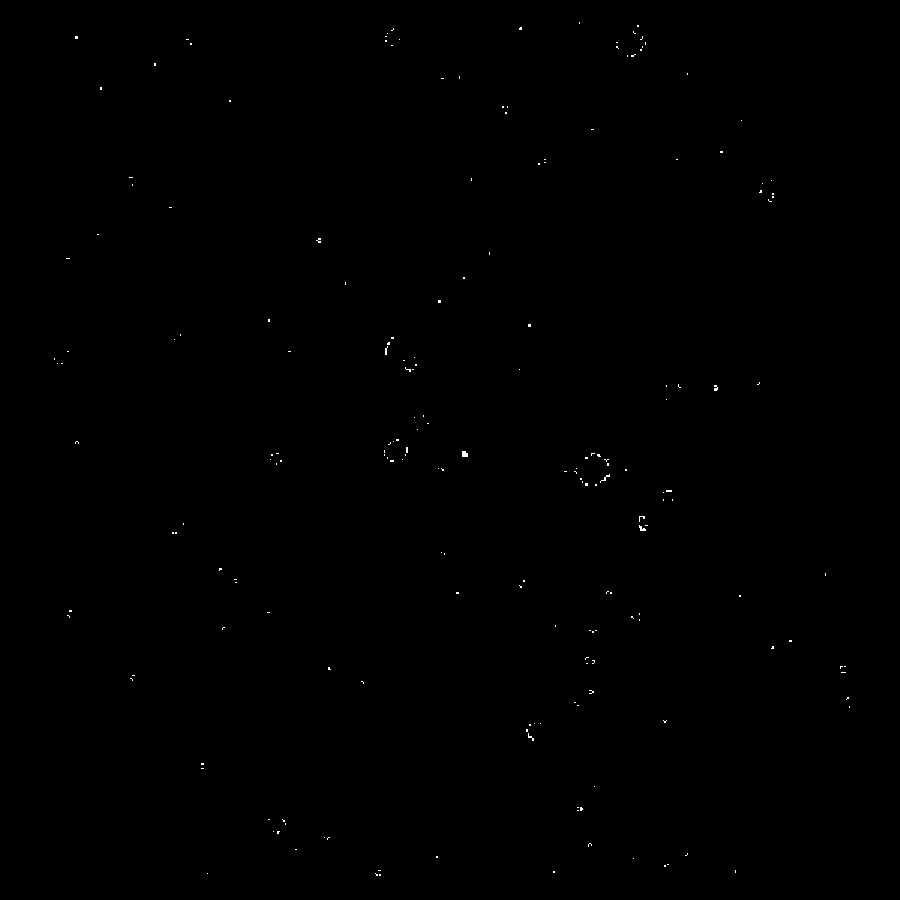
\includegraphics[width=0.33\textwidth]{Figures/NEATImageDiff2.pdf} &
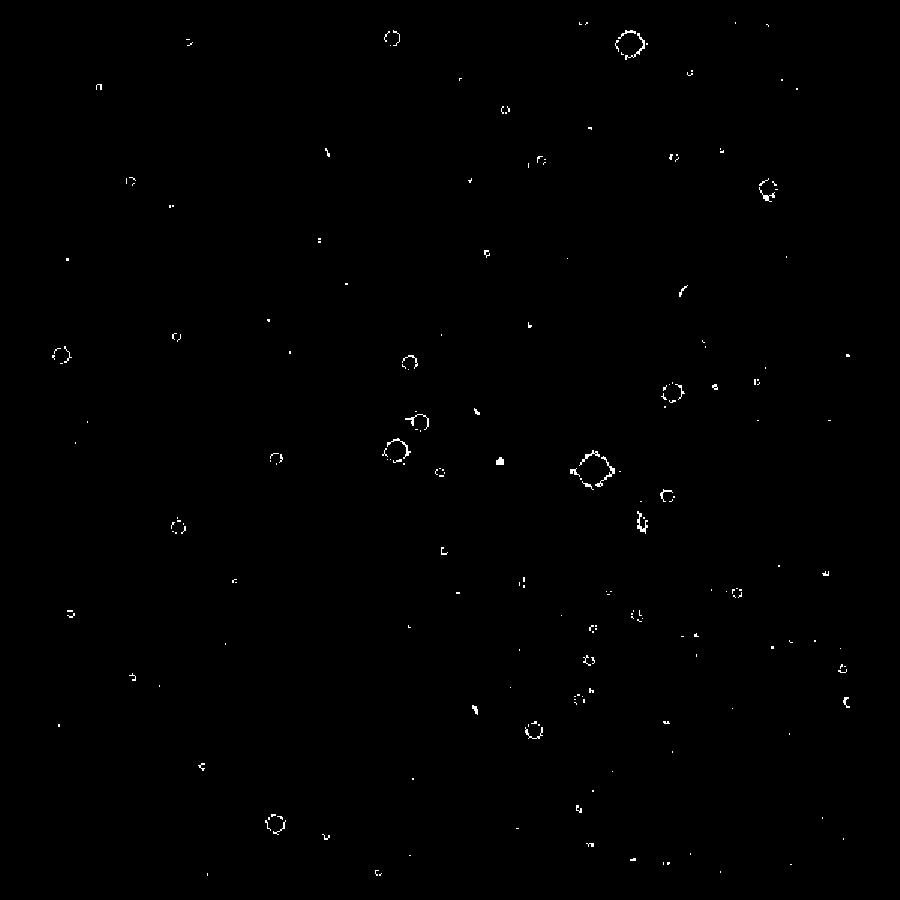
\includegraphics[width=0.33\textwidth]{Figures/NEATImageDiff3.pdf} \\
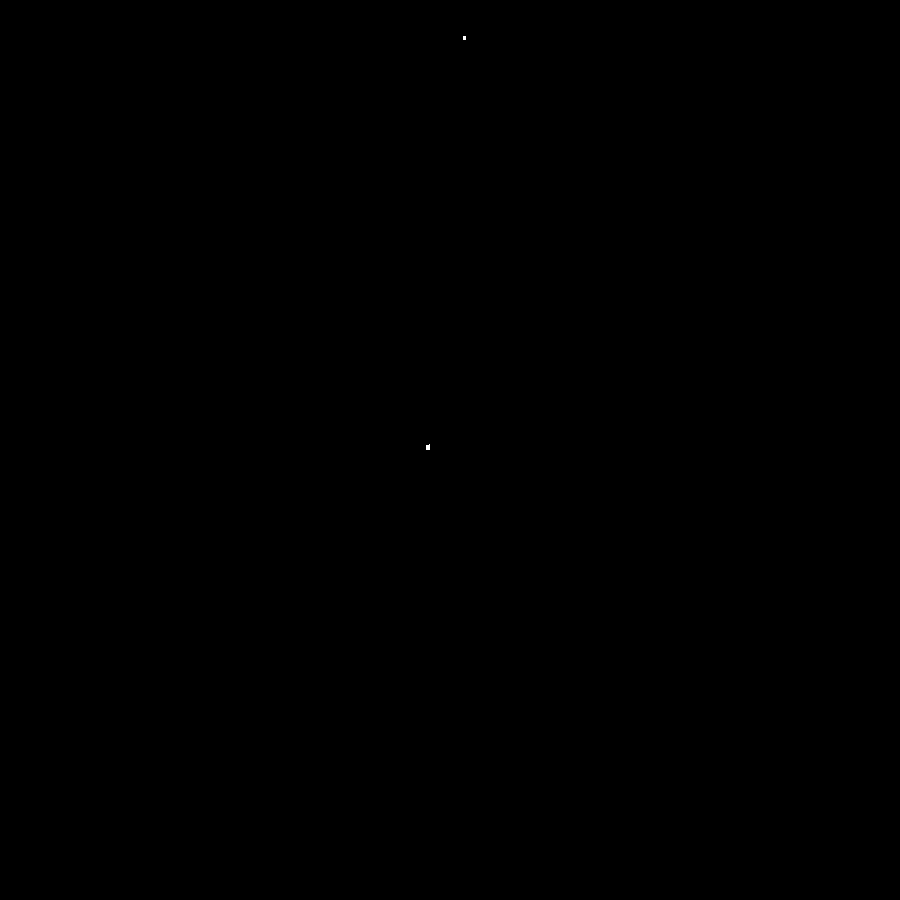
\includegraphics[width=0.33\textwidth]{Figures/NEATFilteredCentroids1.pdf} &
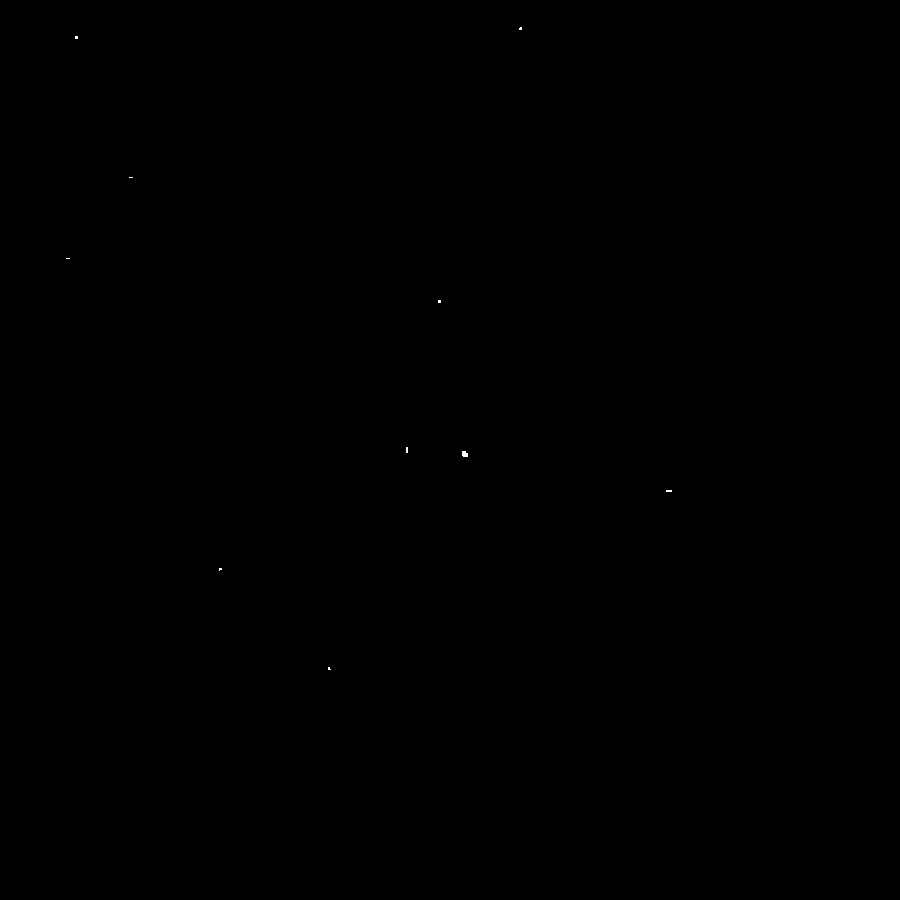
\includegraphics[width=0.33\textwidth]{Figures/NEATFilteredCentroids2.pdf} &
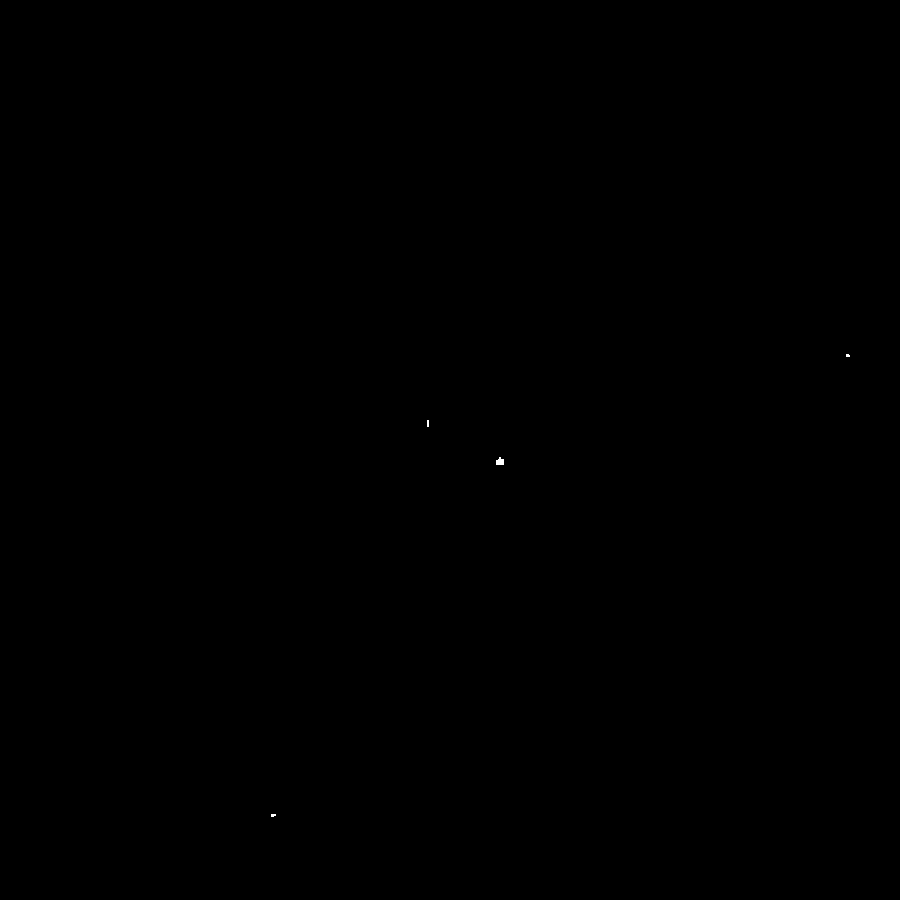
\includegraphics[width=0.33\textwidth]{Figures/NEATFilteredCentroids3.pdf}
\end{array}$
\end{center}
\caption{Option 3. Image Processing Pipeline results. 
First column: 2002 CY46 Triplet images taken 10 minutes apart. Near Earth Asteroid Tracking (NEAT) system archive. 
Second Column: Image Registration results for the CY46 Triplet.  Top: Image-1 registered to Image-2. Middle: Image-2 Bottom: Image-3 registered to Image-2.
Third Column: Image Differencing results for the CY46 Triplet. (Artifacts such as crater-like formations are seen in the difference images above. This is the result of some celestial bodies being over-exposed.) 
Fourth Column: Image Differencing results for the CY46 Triplet. Filtered centroids in each image of the sequence.)}
\end{figure*}

%\begin{figure}[b]
%\minipage{0.24\textwidth}
%  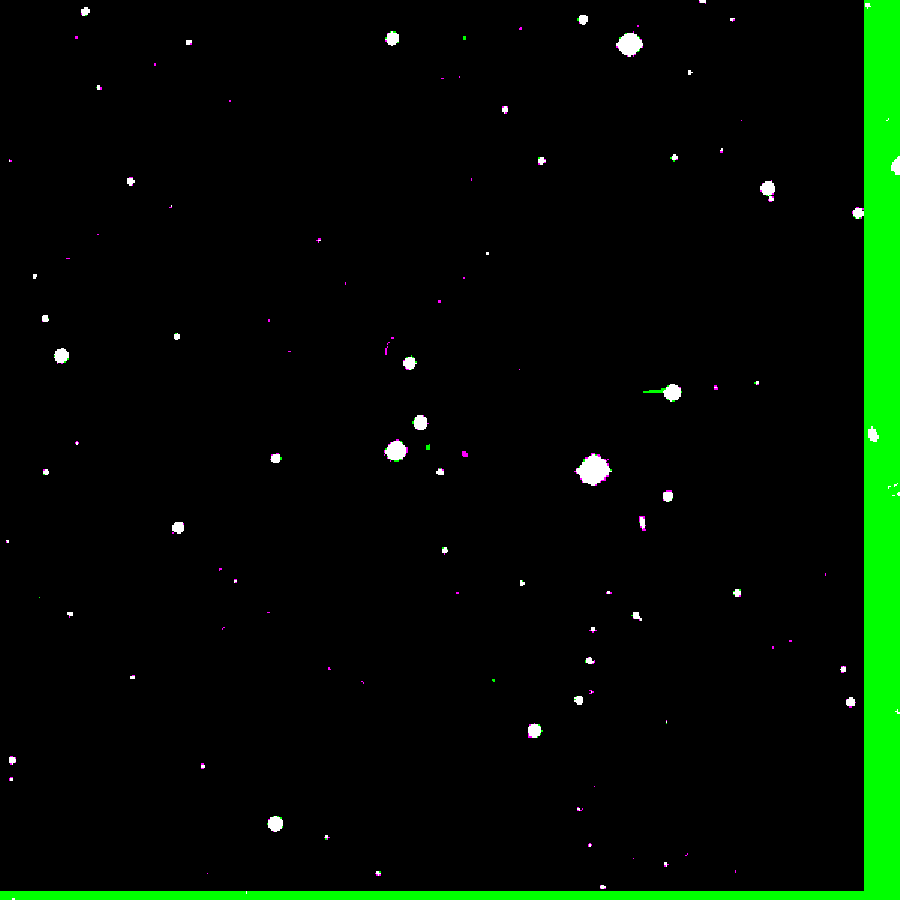
\includegraphics[width=\linewidth]{Figures/NEATImageReg12.pdf}
%\endminipage\hfill
%\minipage{0.24\textwidth}
%  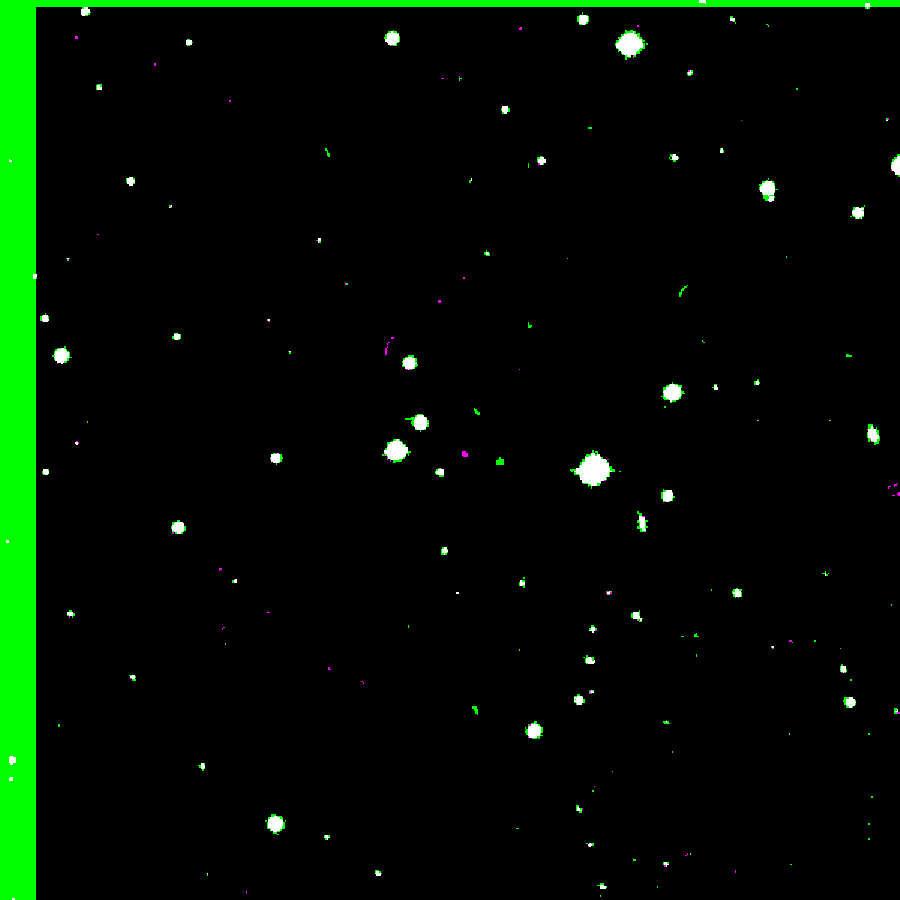
\includegraphics[width=\linewidth]{Figures/NEATImageReg32.pdf}
%\endminipage\hfill
%\caption{Image Registration results for the CY46 Triplet.  Left: Image-1 registered to Image-2. Right: Image-3 registered to Image-2.}
%\label{fig:NEAT_Registration}
%\end{figure}

%\begin{figure*}
%\minipage{0.33\textwidth}
%  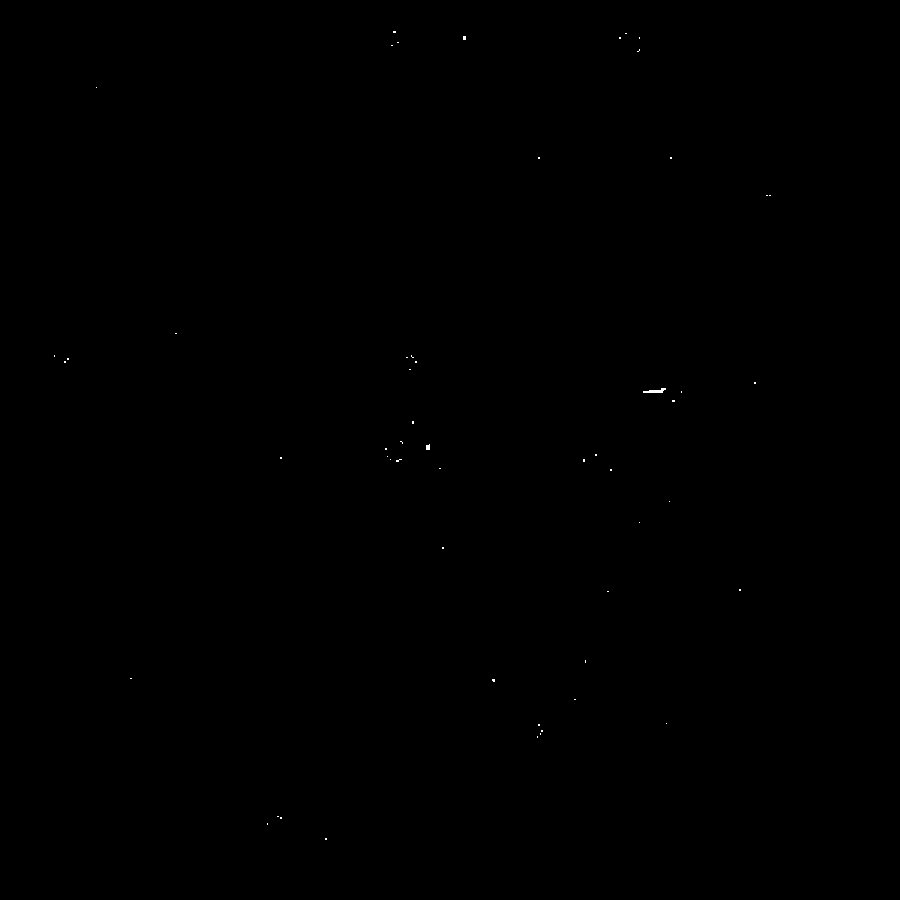
\includegraphics[width=\linewidth]{Figures/NEATImageDiff1.pdf}
%\endminipage\hfill
%\minipage{0.33\textwidth}
%  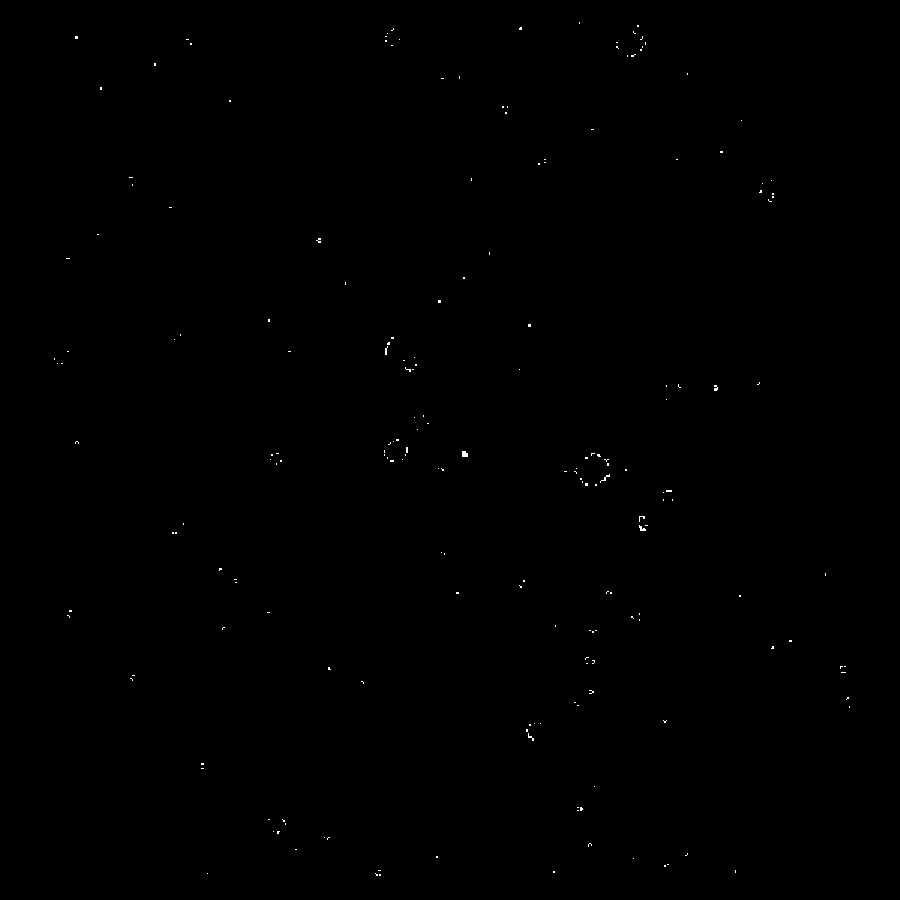
\includegraphics[width=\linewidth]{Figures/NEATImageDiff2.pdf}
%\endminipage\hfill
%\minipage{0.33\textwidth}
%  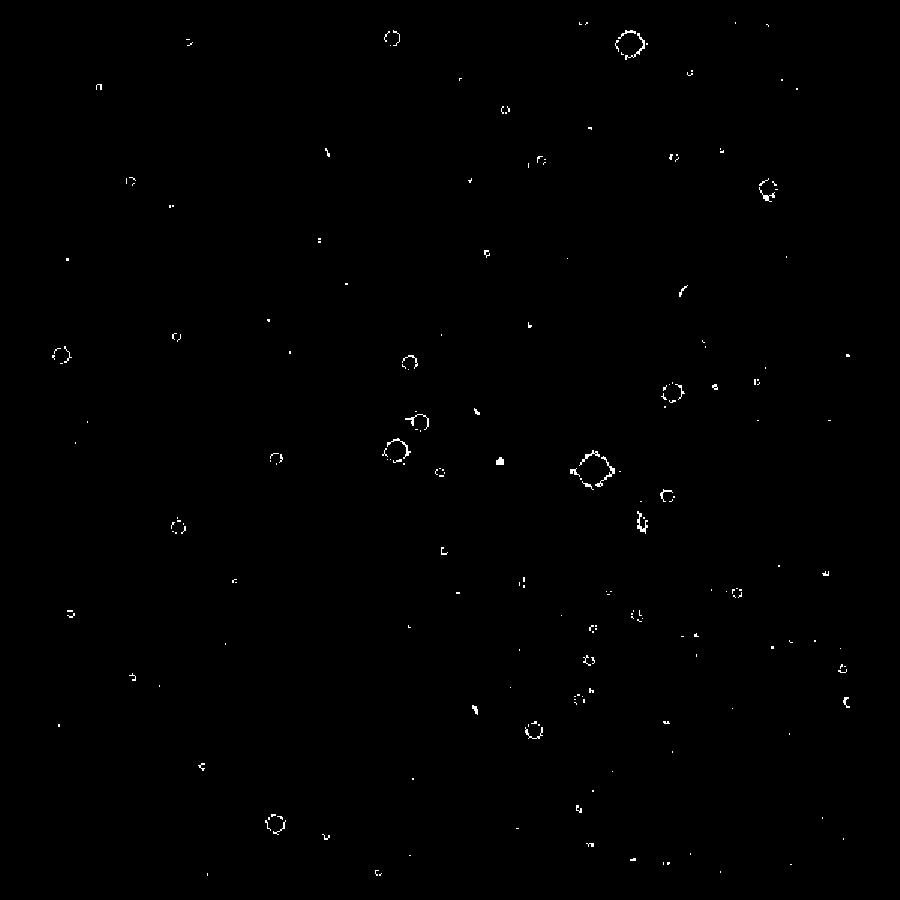
\includegraphics[width=\linewidth]{Figures/NEATImageDiff3.pdf}
%\endminipage
%\caption{Image Differencing results for the CY46 Triplet. (Artifacts such as crater-like formations are seen in the difference images above. This is the result of some celestial bodies being over-exposed.)}
%\label{fig:NEAT_ImgDiff1}
%\end{figure*}

%\begin{figure*}
%\minipage{0.33\textwidth}
%  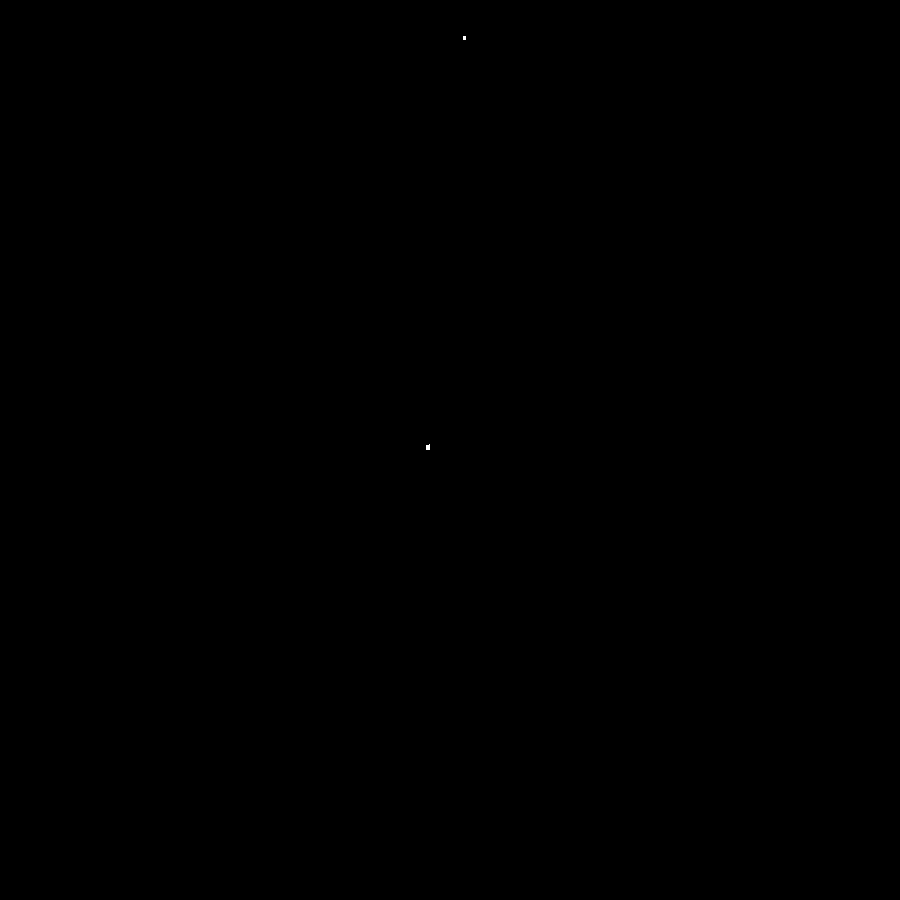
\includegraphics[width=\linewidth]{Figures/NEATFilteredCentroids1.pdf}
%\endminipage\hfill
%\minipage{0.33\textwidth}
%  \includegraphics[width=\linewidth]{Figures/NEATFilteredCentroids2.pdf}
%\endminipage\hfill
%\minipage{0.33\textwidth}
%  \includegraphics[width=\linewidth]{Figures/NEATFilteredCentroids3.pdf}
%\endminipage
%\caption{Image Differencing results for the CY46 Triplet. Filtered centroids in each image of the sequence.)}
%\label{fig:NEAT_ImgDiff2}
%\end{figure*}

\begin{figure}[h]
%\minipage{0.40\textwidth}
%  \includegraphics[width=\linewidth]{Figures/NEATLines_LogicalImg.pdf}
%\endminipage\hfill
\begin{center}
\includegraphics[width=0.4\textwidth]{Figures/NEATLines_LogicalImg.pdf}
\end{center}
\caption{Trajectory Detection for the CY46 Triplet. (Asteroid trajectory detected is shown in green. True location is in red. 3 Images of the triplet are super-imposed here after registration and thresholding for ease of visualization.)}
\label{fig:NEAT}
\end{figure}
\subsubsection{CATALINA}


\subsection{performance characterization}
We use the following metrics for algorithm testing and validation.  These are used to characterize the performance of the algorithm for the three successive stages: the initial detection of objects, the detection of moving objects and the detection of trajectories:
1.	Precision: The fraction of retrieved/detected objects (celestial bodies, moving objects, trajectories) that are relevant, i.e. correspond to correct detections.
2.	Recall: The fraction of relevant (true) objects (celestial bodies, moving objects, trajectories) that are actually detected/retrieved.
3.	Receiver Operating Characteristic (ROC): A plot of the probability of detection as a function of the probability of false alarm generated by varying a significant parameter of the algorithm (such as the initial detection threshold).  This will detail the performance of the system as the parameters of the image processing pipeline are varied. 
4.	Area under the ROC curve (AUC) that characterizes the performance of detection vs. false alarm with a single metric.
5.	Localization error: For those correctly detected asteroids, we will characterize the localization error by computing the 3D (angular pointing error).  The simulation and the test image sets have the ground truth location of the asteroid in image coordinates.  This true location is compared with the detected trajectory to determine localization error.

The above measures are computed and aggregated over a corpus of images corresponding to a simulated platform and camera.
\subsection{Footprint characterization}
include here some information to the effect that this algorithm is deployable on a reference platform.
Efforts are currently being conducted to translate this algorithm in ...